% !TEX root = ./document.tex

\documentclass[a4paper, spanish]{article}

\usepackage{mystyle}
\usepackage{myvars}

\begin{document}

  \maketitle

  \begin{abstract}
		\noindent El objetivo de este trabajo es el análisis de una serie temporal univariante. En este caso, se utilizan modelos \emph{SARIMA}, los cuales se refieren a la extensión con estacionalidad de modelos \emph{ARIMA}. Estos permiten la modelización de series temporales a partir de combinaciones lineales de la componente determinista (parte autoregresiva) y la componente estocástica (parte de media móvil) de la serie. Para el análisis se utilizará la serie \texttt{weightloss}.
	\end{abstract}

  \begin{itemize}
    \item \textbf{Archivo}: \texttt{weight-loss.csv}
    \item \textbf{Serie}: Frecuencia de búsquedas para la palabra clave \say{Weight loss} a través del buscador \emph{Google} por meses, desde \emph{Enero de 2004} hasta \emph{Diciembre de 2018}. Los valores han sido estandarizados en el rango $[0, 100]$.
  \end{itemize}

  \section{Etapa de identificación}
  \label{sec:1}

    \subsection{Contexto}
    \label{sec:context}

      \paragraph{}
      Tal y como se indica al comienzo de este documento, se va a analizar la serie temporal referida a la frecuencia de búsqueda de la palabra clave \say{Weight loss} (a nivel mundial) a través del buscador \emph{Google}. Se ha escogido esta serie para el trabajo por su componente estacional claramente marcada. Se cree que esta está está estrechamente relacionada con un índice sobre la preocupación de la población por su peso a lo largo del tiempo.

      \paragraph{}
      Para evitar problemas de privacidad, los datos se proporcionan estandarizados en el rango $[0, 100]$, lo cual elimina la escala de los mismos y únicamente permite estudiar la estructura de la serie. Esto no es un problema para el análisis que se realizará en este trabajo, dado que precisamente el objetivo del mismo es el de analizar la estructura de una serie serie temporal, siguiendo la metodología de \emph{Box-Jenkins}.

      \paragraph{}
      En cuanto al particionamiento de los datos, estos se proporcionan en agrupaciones mensuales. Dado que se tiene información desde \emph{Enero de 2004} hasta \emph{Diciembre de 2018}, es decir, un total de \emph{15 años}, lo cual suma $15 * 12 = 180$ observaciones en total. Con esta cantidad de observaciones, se cree que se podrá construir un modelo \emph{SARIMA} (\emph{ARIMA} con estacionalidad) de manera adecuada.

      \paragraph{}
      Una vez introducido el contexto de los datos pertenecientes a la serie que se analizará, lo siguiente es empezar a describir la misma a nivel de su estructura estocástica. Tras describir la misma, se procederá a realizar las diferenciaciones pertinentes hasta conseguir que esta sea estacionaria. Una vez se haya conseguido transformar la serie en estacionaria, se tratarán de identificar los parámetros de la parte autoregresiva y de la parte de media móvil, tanto de la dependencia entre observaciones a nivel serial (cada observación con las anteriores), como de la dependencia estacional (cada observación con las anteriores dentro de su periodo estacional). Tras dicha descripción, se propondrán un conjunto de modelos \emph{SARIMA}. En la \autoref{sec:fitting} se prodecerá al ajuste de dichos modelos a los datos. Posteriormente, en la \autoref{sec:comparison} serán descartados aquellos modelos que no puedan validarse por su excesiva falta de ajuste, sobre ajuste, parámetros no significativos, etc. De entre los modelos válidos, se seleccionará aquel cuyo ajuste sea el más próximo a los datos, lo cual se comprobará mediante distintas técnicas. Finalmente, en la \autoref{sec:prediction} se realizará una predicción para el próximo año (\emph{2019}) sobre los valores esperados por el modelo seleccionado.

      \paragraph{}
      La metodología que se ha expuesto en el párrafo anterior se corresponde con la propuesta por \emph{Box-Jenkins} para series temporales basada en ajuste de modelos \emph{ARIMA}. En el documento, se sigue un enfoque en paralelo en lugar de iterativo para la búsqueda del mejor modelo para facilitar la interpretación y la organización del mismo. Esta es la única modificación que se ha llevado a cabo respecto de la metodología original.

    \subsection{Análisis Descriptivo}
    \label{sec:descriptive}


      \paragraph{}
      Tras la descripción de la metodología, se va a comenzar con la descripción de la serie temporal. Para ello, nos vamos a apoyar en los gráficos de la \autoref{img:weightloss}, a partir de los cuales se puede tener una perspectiva completa acerca de la serie. A través de ella se puede ver el gráfico de la serie, el correlograma, el correlograma parcial, el periodograma y el diagrama de dispersión \emph{rango-media}.

      \paragraph{}
      En el gráfico de la serie de la \autoref{img:weightloss} se puede apreciar la evolución temporal de los valores a lo largo de los 15 años, separados en observaciones mensuales. En dicha representación destacan dos características de la serie temporal sobre el resto. Estas son:
        \begin{enumerate*}[label=(\arabic*)]
          \item la marcada estructura estacional de periodo 12 (anual) de la serie, que sigue la misma forma en todas las estacionalidades (años). Esto es un fuerte crecimiento durante el primer mes (Enero), posteriormente se produce un suave decrecimiento hasta el tercer cuarto del año, para producirse un fuerte decrecimiento en torno a los meses de Septiembre - Octubre. Esta estructura estacional es coherente con el fenómeno conocido como \emph{Operación Bikini}, que consiste en la preocupación por estar en buena forma física durante los meses de verano. Esta preocupación comienza en torno a principios de año y se mantiene hasta los meses de verano. Puesto que una vez pasados dichos meses, la forma física deja de estar comprometida, la preocupación por la pérdida de peso de la población también disminuye.
          \item el cambio de nivel que se produce entre el año $2008$ y el año $2009$. Durante este periodo se produce un cambio drástico en el nivel de la serie. Parece que durante el final del año $2008$ no se produjo el fenómeno esperado de un fuerte decrecimiento que sí se produce durante el resto de años. Este cambio en el nivel de la serie pudo deberse a distintos factores. Uno de ellos pudo ser la crisis económica cuyas evidencias comonezaron en torno a dicho año. Si se confirmase que las razones del aumento del nivel en las búsquedas del término \emph{Weight loss} fueron debidas a la crisis económica, una interpretación para la misma podría ser la siguiente: Con el aumento del riesgo en la estabilidad financiera, la población aumentó también su preocupación en su apariencia física, lo cual se ha mantenido hasta la actualidad. Otro de los factores de peso pudo haber sido el acercamiento de la tecnología y redes sociales a la mayoría de la población, que hasta entonces se había mantenido alejada de ella. Dado que muchas redes sociales permiten la posibilidad de incluir imágenes personales que otras personas pueden juzgar, el índice de preocupación por el nivel de forma física puede haberse incrementado en los últimos años debido a dicha razón. Sin embargo, estas interpretaciones queda fuera del objetivo de este trabajo.
        \end{enumerate*}

      \begin{figure}[htb!]
        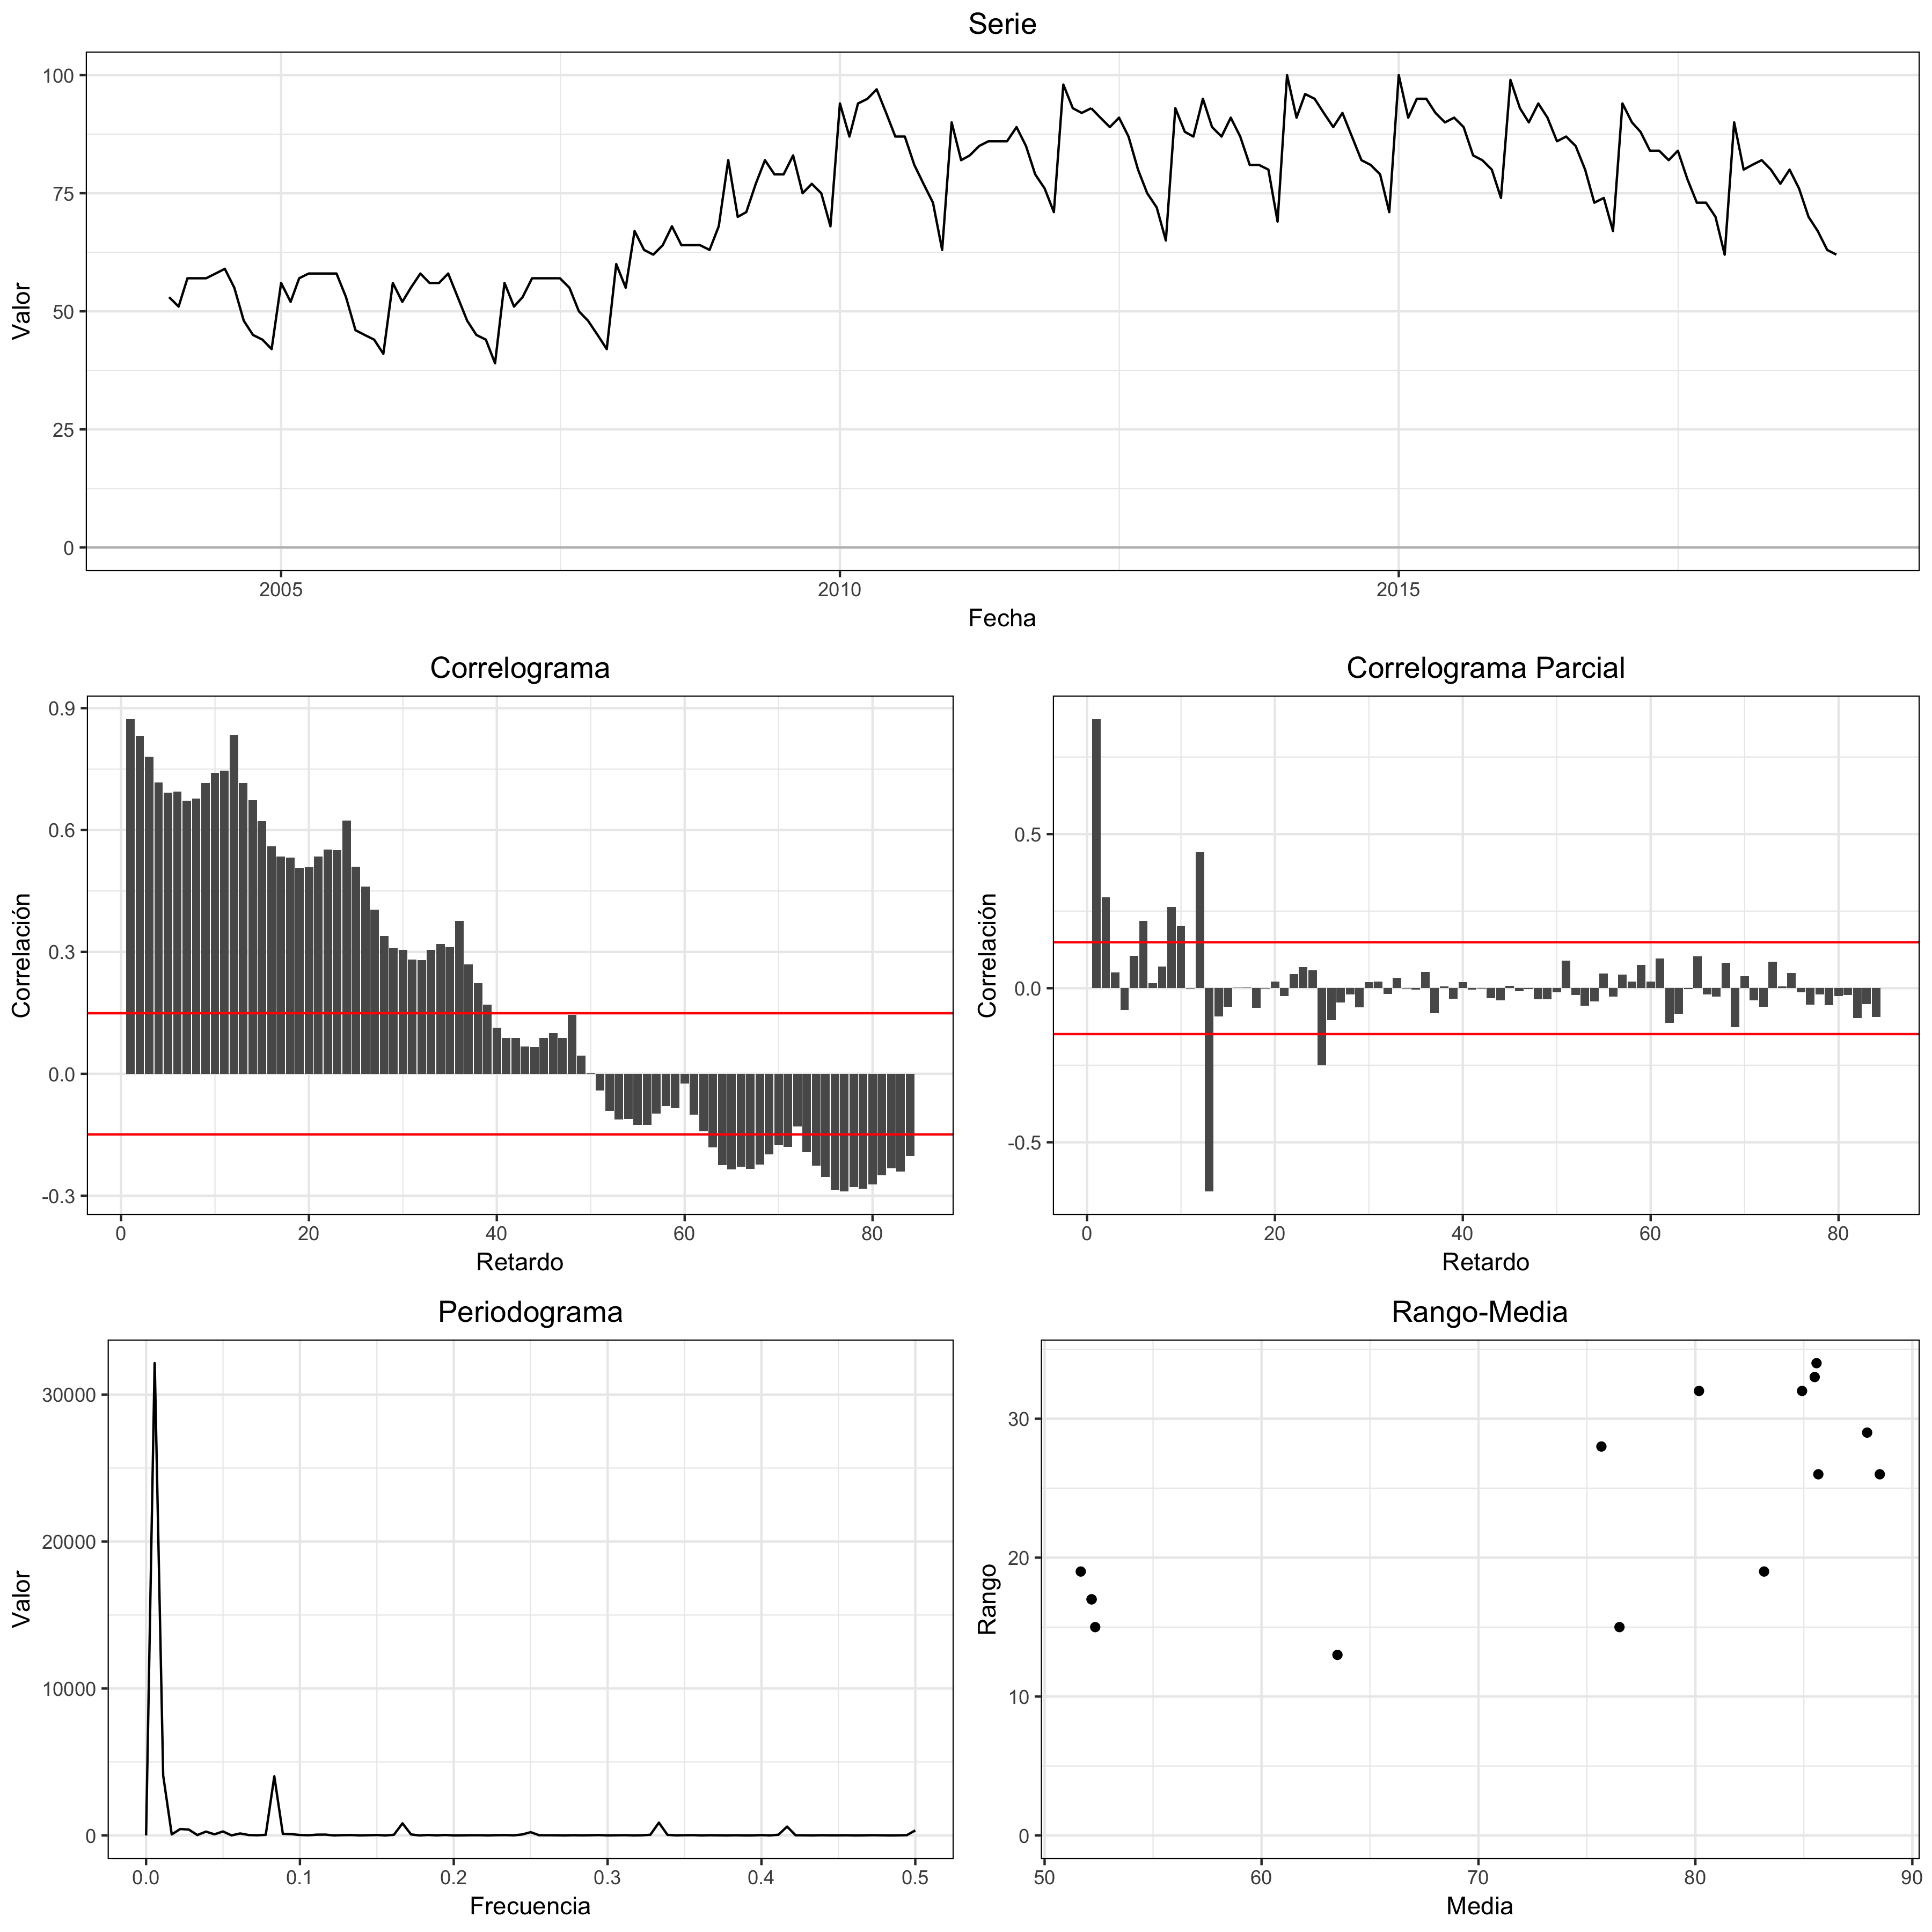
\includegraphics[width=\textwidth,height=\textheight,keepaspectratio]{weightloss}
        \caption{Gráfico de la serie, Correlograma, Correlograma Parcial, Periodograma y diagrama de dispersión \emph{rango-media} para la serie \texttt{weightloss}.}
        \label{img:weightloss}
      \end{figure}

      \paragraph{}
      En cuanto al correlograma de la serie que se muestra en la \autoref{img:weightloss}, se puede apreciar la componente estacional de periodo 12 en la estructura de correlaciones. Destacan sobre el resto los retardos de la forma $i \text{ mod } 12 = 0$, estos son los retardos $12, 24, 36,...$. Estos se relacionan entre si presentando un decrecimiento lineal, por lo que son indicativo de que la serie no es estacionaria. Por lo tanto, tendremos que llevar a cabo al menos una diferenciación estacional para conseguir estacionarizar la serie. También llama la atención la gran cantidad de correlaciones con valores significativos, por lo que la tendencia podría estar ocultando algún otro comportamiento no visible a simple vista. Por lo tanto, la realización de una diferenciación regular también podría ser una buena estrategia para tratar de comprender en mayor medida la estructura de correlaciones de la serie. Como se verá en el siguiente párrafo, estas interpretaciones se ven reflejadas en el correlograma parcial.

      \paragraph{}
      En el correlograma parcial de la serie de la \autoref{img:weightloss} se representan las correlaciones entre observaciones de la serie, tratando de eliminar de estas la relación procedente de otros retardos. Es decir, el correlograma parcial trata de representar de manera aislada la correlación entre una observación y la del $k$-ésimo retardo posterior, eliminando la influencia del resto. En este caso destacan sobre el resto los retardos $1$, $12$ y $13$. Se cree que el retardo $1$ destaca sobre el resto debido a la tendencia de la serie mientras que el retardo $12$ se debe a la estacionalidad de la misma. También se piensa que el retardo $13$ es un reflejo del $1$, en la estacionalidad anterior, de ahí la razón de que destaque de tal manera.

      \paragraph{}
      En cuanto al periodograma de la serie que se muestra en la \autoref{img:weightloss}, se puede apreciar que el primer armónico recoge gran parte de la variabilidad de la serie, lo cual de nuevo vuelve a indicar que la tendencia de la misma puede estar ocultando información sobre la estructura estocástica de la serie. Por lo tanto, se cree que una diferenciación permitiría visualizar en mayor medida el comportamiento de la misma. También destacan (aunque de una manera mucho menos pronunciada) los armónicos de la forma $i + 1 / 12$ con $i \in {1, 2, ..., 6}$, esto es $1/12, 2/12, ..., 6/12$, lo cual es otro argumento de peso en favor de la componente estacional de periodo $12$ (anual) de la serie.

      \paragraph{}
      En cuanto al diagrama de dispersión \emph{rango-media} de la \autoref{img:weightloss}, parece que exista una leve relación entre el nivel de la serie y la dispersión del mismo. Este fenómeno podría requerir de alguna transfomación de estabilización de varianza, como las de la forma \emph{Box-Cox}. La razón de ello es que los modelos que se ajustarán a la serie temporal requieren de estacionaridad en la serie (entre otros requisitos, la varianza debe ser constante a lo largo de la serie). Sin embargo, tal y como se verá posteriormente, las diferenciaciones eliminarán la relación entre nivel y dispersión, por lo que es algo de lo que no nos preocuparemos en gran medida.


    \subsection{Diferenciaciones}
    \label{sec:differences}

      \paragraph{}
      Anteriormente, se ha realizado un análisis descriptivo acerca de la estructura de la serie \texttt{weightloss}, tras el cual se llegó a la conclusión de que la serie no presentaba la propiedad de estacionaridad (nivel y estructura de correlaciones constante para todas las observaciones). Por tanto, se indicó que para llegar a una serie estacionaria, la solución sería encontrar una diferenciación o varias diferenciaciones que transformen la serie en estacionaria.

      \paragraph{}
      Tal y como se indicó anteriormente, para conseguir la propiedad de estacionaridad dichas diferenciaciones podrían ser de dos tipos: \begin{enumerate*}[label=(\arabic*)]
        \item diferenciación regular para reducir la componente de tendencia de la serie, y
        \item diferenciación estacional de periodo 12 para reducir las correlaciones entre observaciones de un mismo índice estacionalidad.
      \end{enumerate*} Entonces, la estrategia a seguir será la de probar entre distintas combinaciones de diferenciaciones (de orden reducido, ya que de no ser así entonces se producirían efectos tales como el aumento de la varianza de la serie).

      \paragraph{}
      Por tanto, para elegir el orden de diferenciación se han probado distintas alternativas. En la \autoref{table:variance_differences} se incluye una relación entre la varianza resultante de las observaciones de la serie y el orden de diferenciación de la misma. Como se puede apreciar, la serie original tiene una varianza de $258.67$. Sin embargo, la de la serie tras aplicar una diferenciación regular y otra estacional es únicamente de $14.07$.

      \begin{table}[htb!]
        \centering
        \begin{tabular}{|l|r|}
            \hline
            \textbf{Serie} & \textbf{Varianza}
            \csvreader[head to column names]{res/data/variance-differences.csv}{}
            {\\ \hline \name & \variance}
            \\\hline
        \end{tabular}
        \caption{Relación entre distintos órdenes de diferenciación y varianza de la serie resultante.}
        \label{table:variance_differences}
      \end{table}

      \paragraph{}
      Tanto por la reducida varianza, como por la propiedad de estacionaridad, finalmente escogerémos los grados de diferenciación $1$ para la componente regular y $1$ para la componente estacional. Sin embargo, a continuación se van a estudiar un poco más en detalle los resultados de la serie tras la aplicación de distintas diferenciaciones: En la \autoref{sec:regular_difference} se analiza la serie diferenciada regularmente y en la \autoref{sec:seasonal_difference} se analiza la serie diferenciada estacionalmente. Por último, en la \autoref{sec:regular_seasonal_difference} se muestra la serie diferenciada tanto regular como estacionalmente. Tal y como se ha indicado anteriormente, esta será la serie con la que se continuará el análisis y posterior ajuste.

      \subsubsection{Diferenciación regular}
      \label{sec:regular_difference}

        \paragraph{}
        La diferenciación regular consiste en la aplicación del operador $\nabla$ una vez a la serie objetivo. Esto es equivalente a multiplicar la misma por el término $(1 - B)$, donde $B$ consiste en el operador \emph{backward}, que genera como resultado la observación anterior. En la \autoref{eq:diff_1} se muestra la representación de la diferenciación regular. Esto consiste en substraer el valor de la observación actual a la anterior. Tras aplicar esta operación a todas las observaciones de la serie, se consigue la eliminación de una tendencia de carácter lineal. Nótese que para hacer esto, se están perdiendo $1$ observación.

        \begin{equation}
        \label{eq:diff_1}
          \begin{split}
            \nabla X_t
            &= (1 - B) \cdot X_t \\
            &= X_t - X_{t-1}
          \end{split}
        \end{equation}

        \paragraph{}
        En la \autoref{img:weightloss_diff_1} se muestran el gráfico de la serie, el correlograma, el correlograma Parcial, el periodograma y el diagrama de dispersión \emph{rango-media} para la serie tras la realización de una diferenciación regular.

        \paragraph{}
        Tal y como se puede apreciar en el gráfico de la serie, se ha eliminado la tendencia de la misma. Ahora la media está en torno al valor $0$, sobre el cual obscila. Sin embargo, se puede apreciar que la serie sigue teniendo una estructura estacional, que la diferenciación no ha podido eliminar. En el correlograma se puede apreciar que dicha estructura de estacionalidad (con las correlaciones múltiplos de 12 claramente marcadas) que estas presentan un decrecimiento de carácter lineal, lo cual indica que la serie no es estacionaria. En el correlograma parcia se puede apreciar la reducción de la correlación del primer retardo, lo cual era algo obvio tras la diferenciación regular. En cuanto al periodograma, ahora se pueden apreciar de una manera muy marcada los armónicos significativos, los cuales siguen la forma $i / 12$. Este es otro de los argumentos en favor de la diferenciación estacional, que se realizará en la \autoref{sec:seasonal_difference}. En cuanto al gráfico de dispersión \emph{rango-media}, se puede comprobar que ahora se ha conseguido controlar en mayor medida la relación entre el nivel y la dispersión, es decir, se ha estabilizado en mayor medida la varianza. Sin embargo, esto se conseguirá en mayor media en las diferenciaciones posteriores.

        \begin{figure}[htb!]
          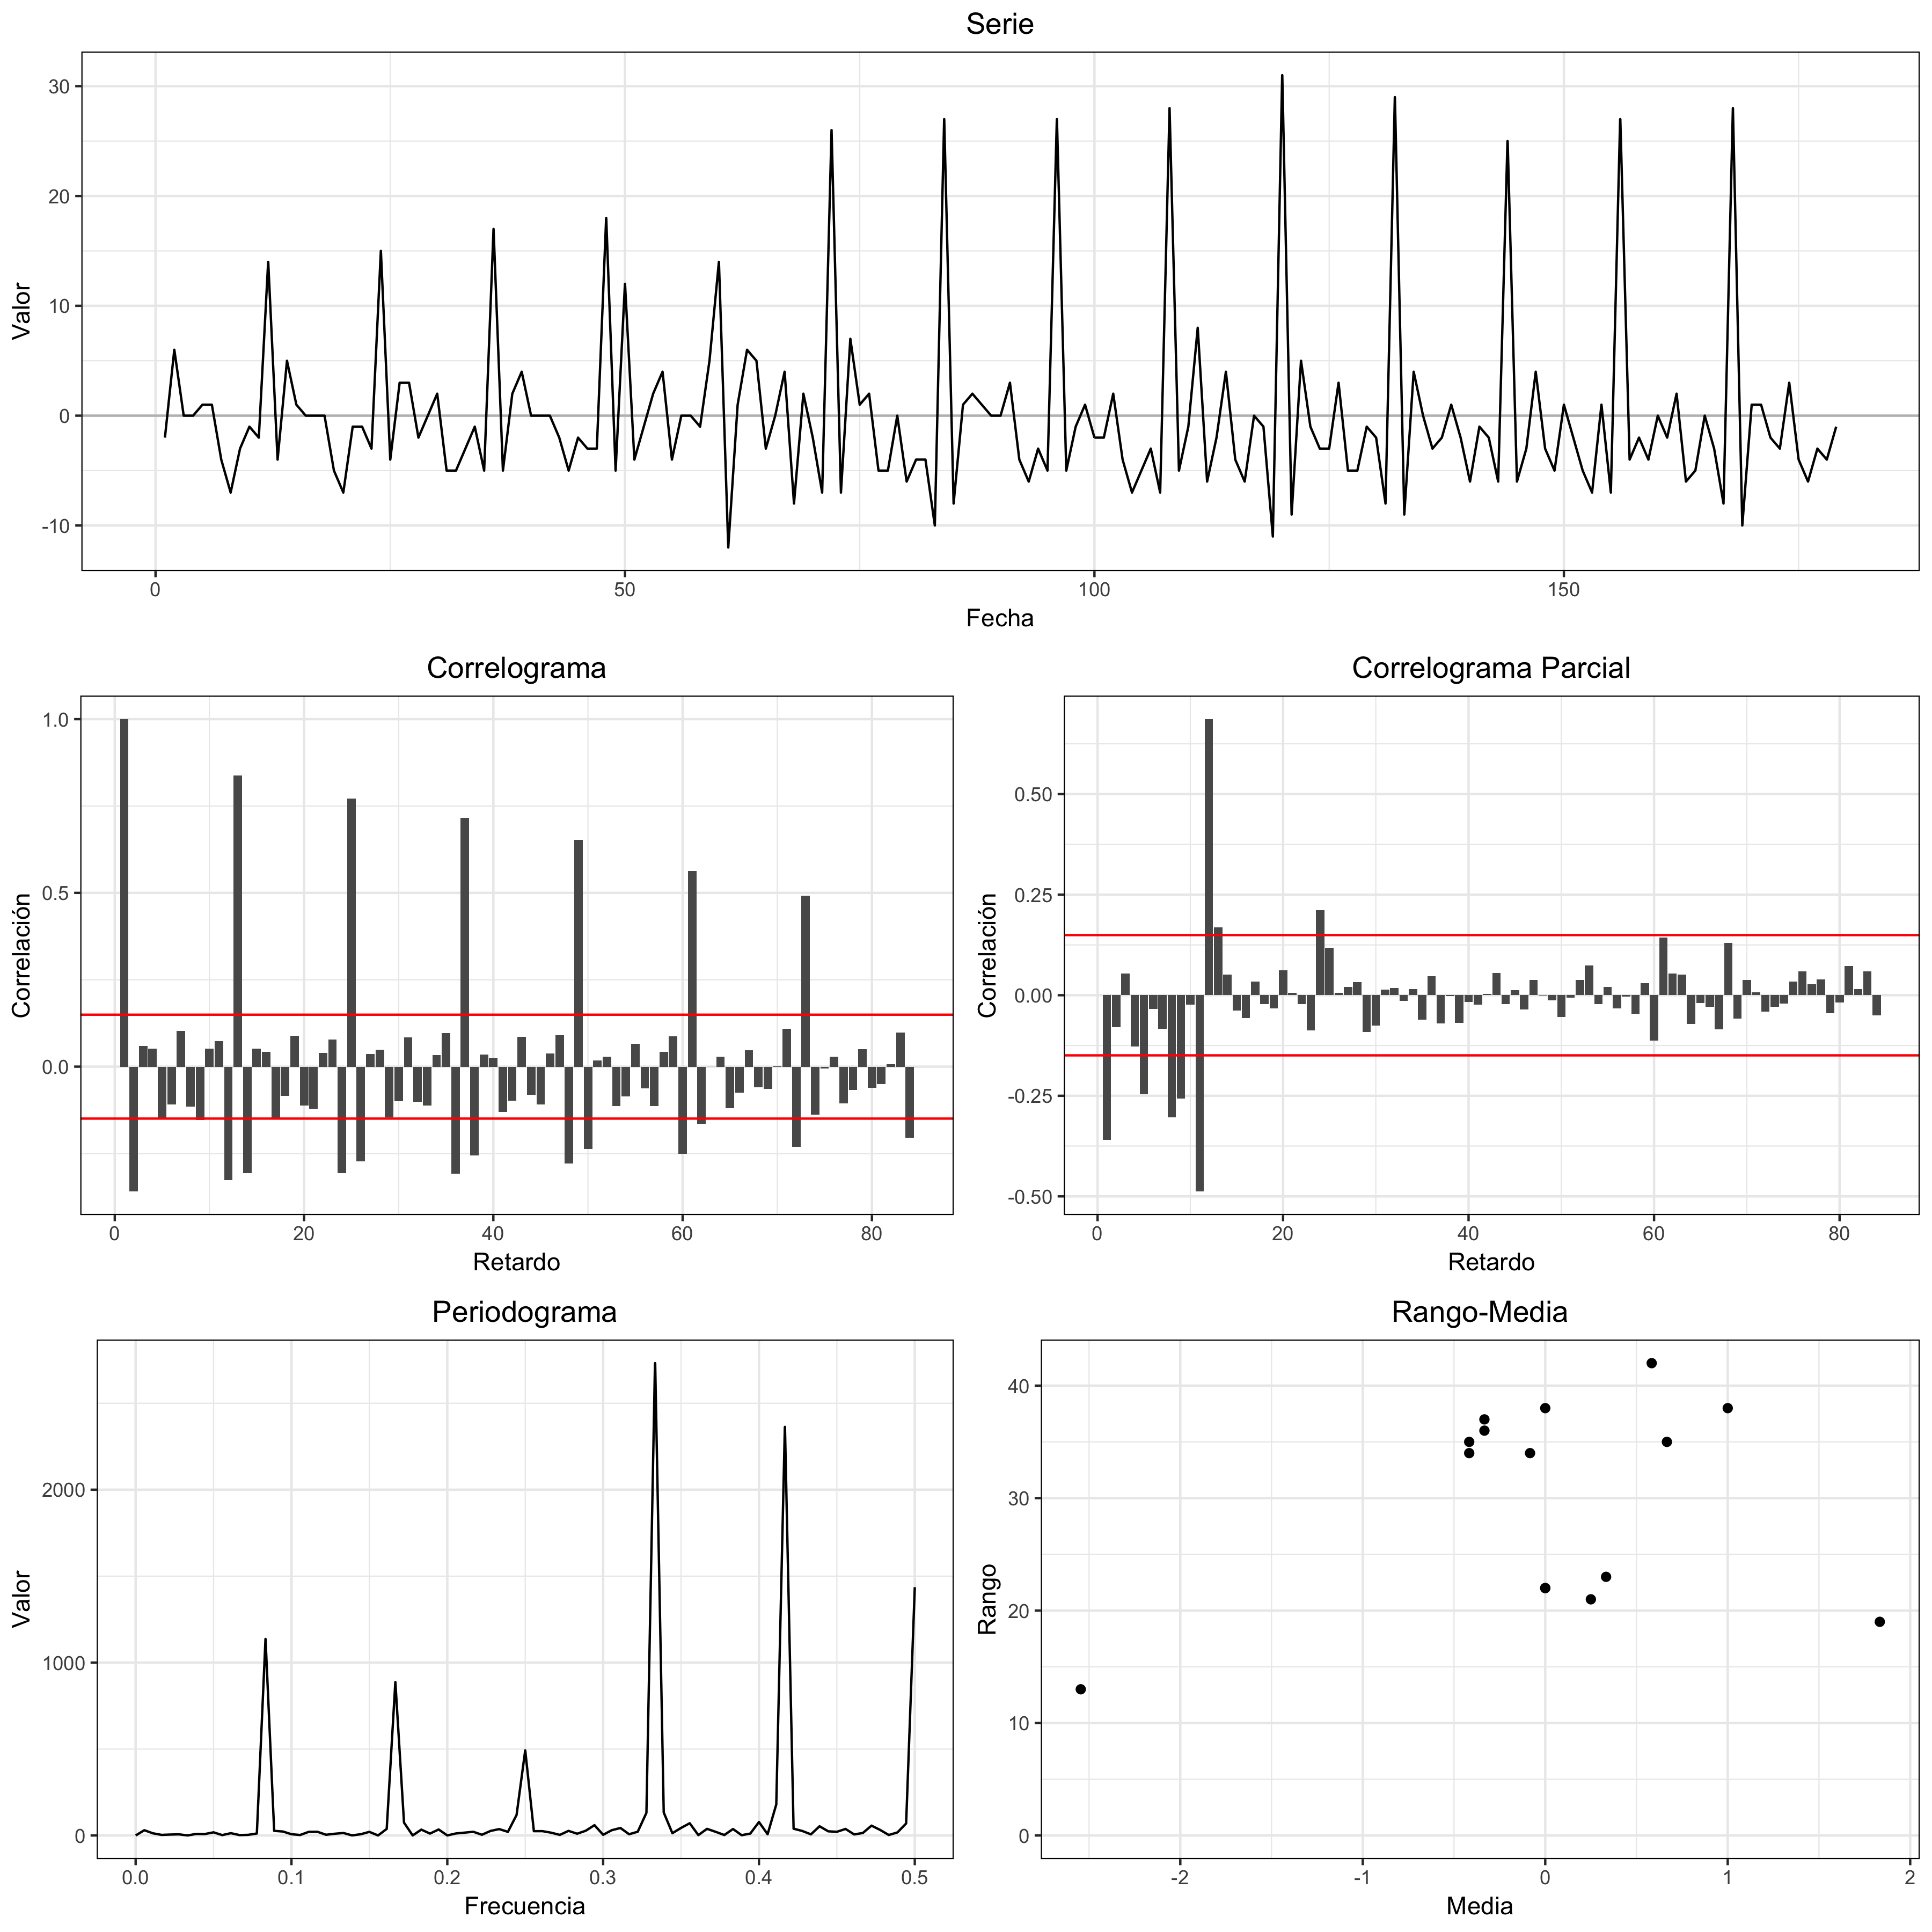
\includegraphics[width=\textwidth,height=\textheight,keepaspectratio]{weightloss-diff-1}
          \caption{Gráfico de la serie, Correlograma, Correlograma Parcial, Periodograma y diagrama de dispersión \emph{rango-media} para la serie \texttt{weightloss} tras la realización de una diferenciación regular.}
          \label{img:weightloss_diff_1}
        \end{figure}

        \paragraph{}
        La aplicación de la una diferenciación regular a la serie \texttt{weightloss} ha repercutido de manera positiva sobre la misma desde el punto de vista de la estacionaridad (ahora se encuentra más cerca de cumplir dicha propiedad). En la \autoref{table:variance_differences} se indica que el valor de la varianza es $62.92$, lo cual es una drástica reducción en la dispersión de la serie. Sin embargo, todavía no puede ser considerada estacionaria. A continuación probaremos la alternativa estacional y estudiaremos los resultados.

      \subsubsection{Diferenciación estacional}
      \label{sec:seasonal_difference}

        \paragraph{}
        La diferenciación estacional se basa en las mismas ideas que la diferenciación regular descrita anteriormente. Sin embargo, en este caso se utiliza una notación de subíndices para indicar el retardo en que aplicar la diferenciación. Esto es, en lugar de substraer de la observación actual la inmediatamente anterior, se substrae la anterior respecto referida al mismo índice estacional. En nuestro caso, esto se refiere a substraer el valor del mismo mes del año anterior, esto es la observación $12$ posiciones hacia atrás. En la \autoref{eq:diff_12} se muestra la expresión de la diferenciación que se acaba de describir. Tal y como se puede apreciar, esta corresponde con la substracción de la observación $12$ posiciones hacia atrás. Si se aplica esta operación a todas las observaciones de la serie, entonces se consigue la serie diferenciada estacionalmente. Nótese que para hacer esto, se están perdiendo $12$ observaciones.

        \begin{equation}
        \label{eq:diff_12}
          \begin{split}
            \nabla_{12} X_t
            &= (1 - B^12) \cdot X_t \\
            &= X_t - X_{t - 12}
          \end{split}
        \end{equation}

        \paragraph{}
        En la \autoref{img:weightloss_diff_12} se muestran el gráfico de la serie, el correlograma, el correlograma parcial, el periodograma y el diagrama de dispersión \emph{rango-media} para la serie tras la realización de una diferenciación estacional (12 retardos).

        \begin{figure}[htb!]
          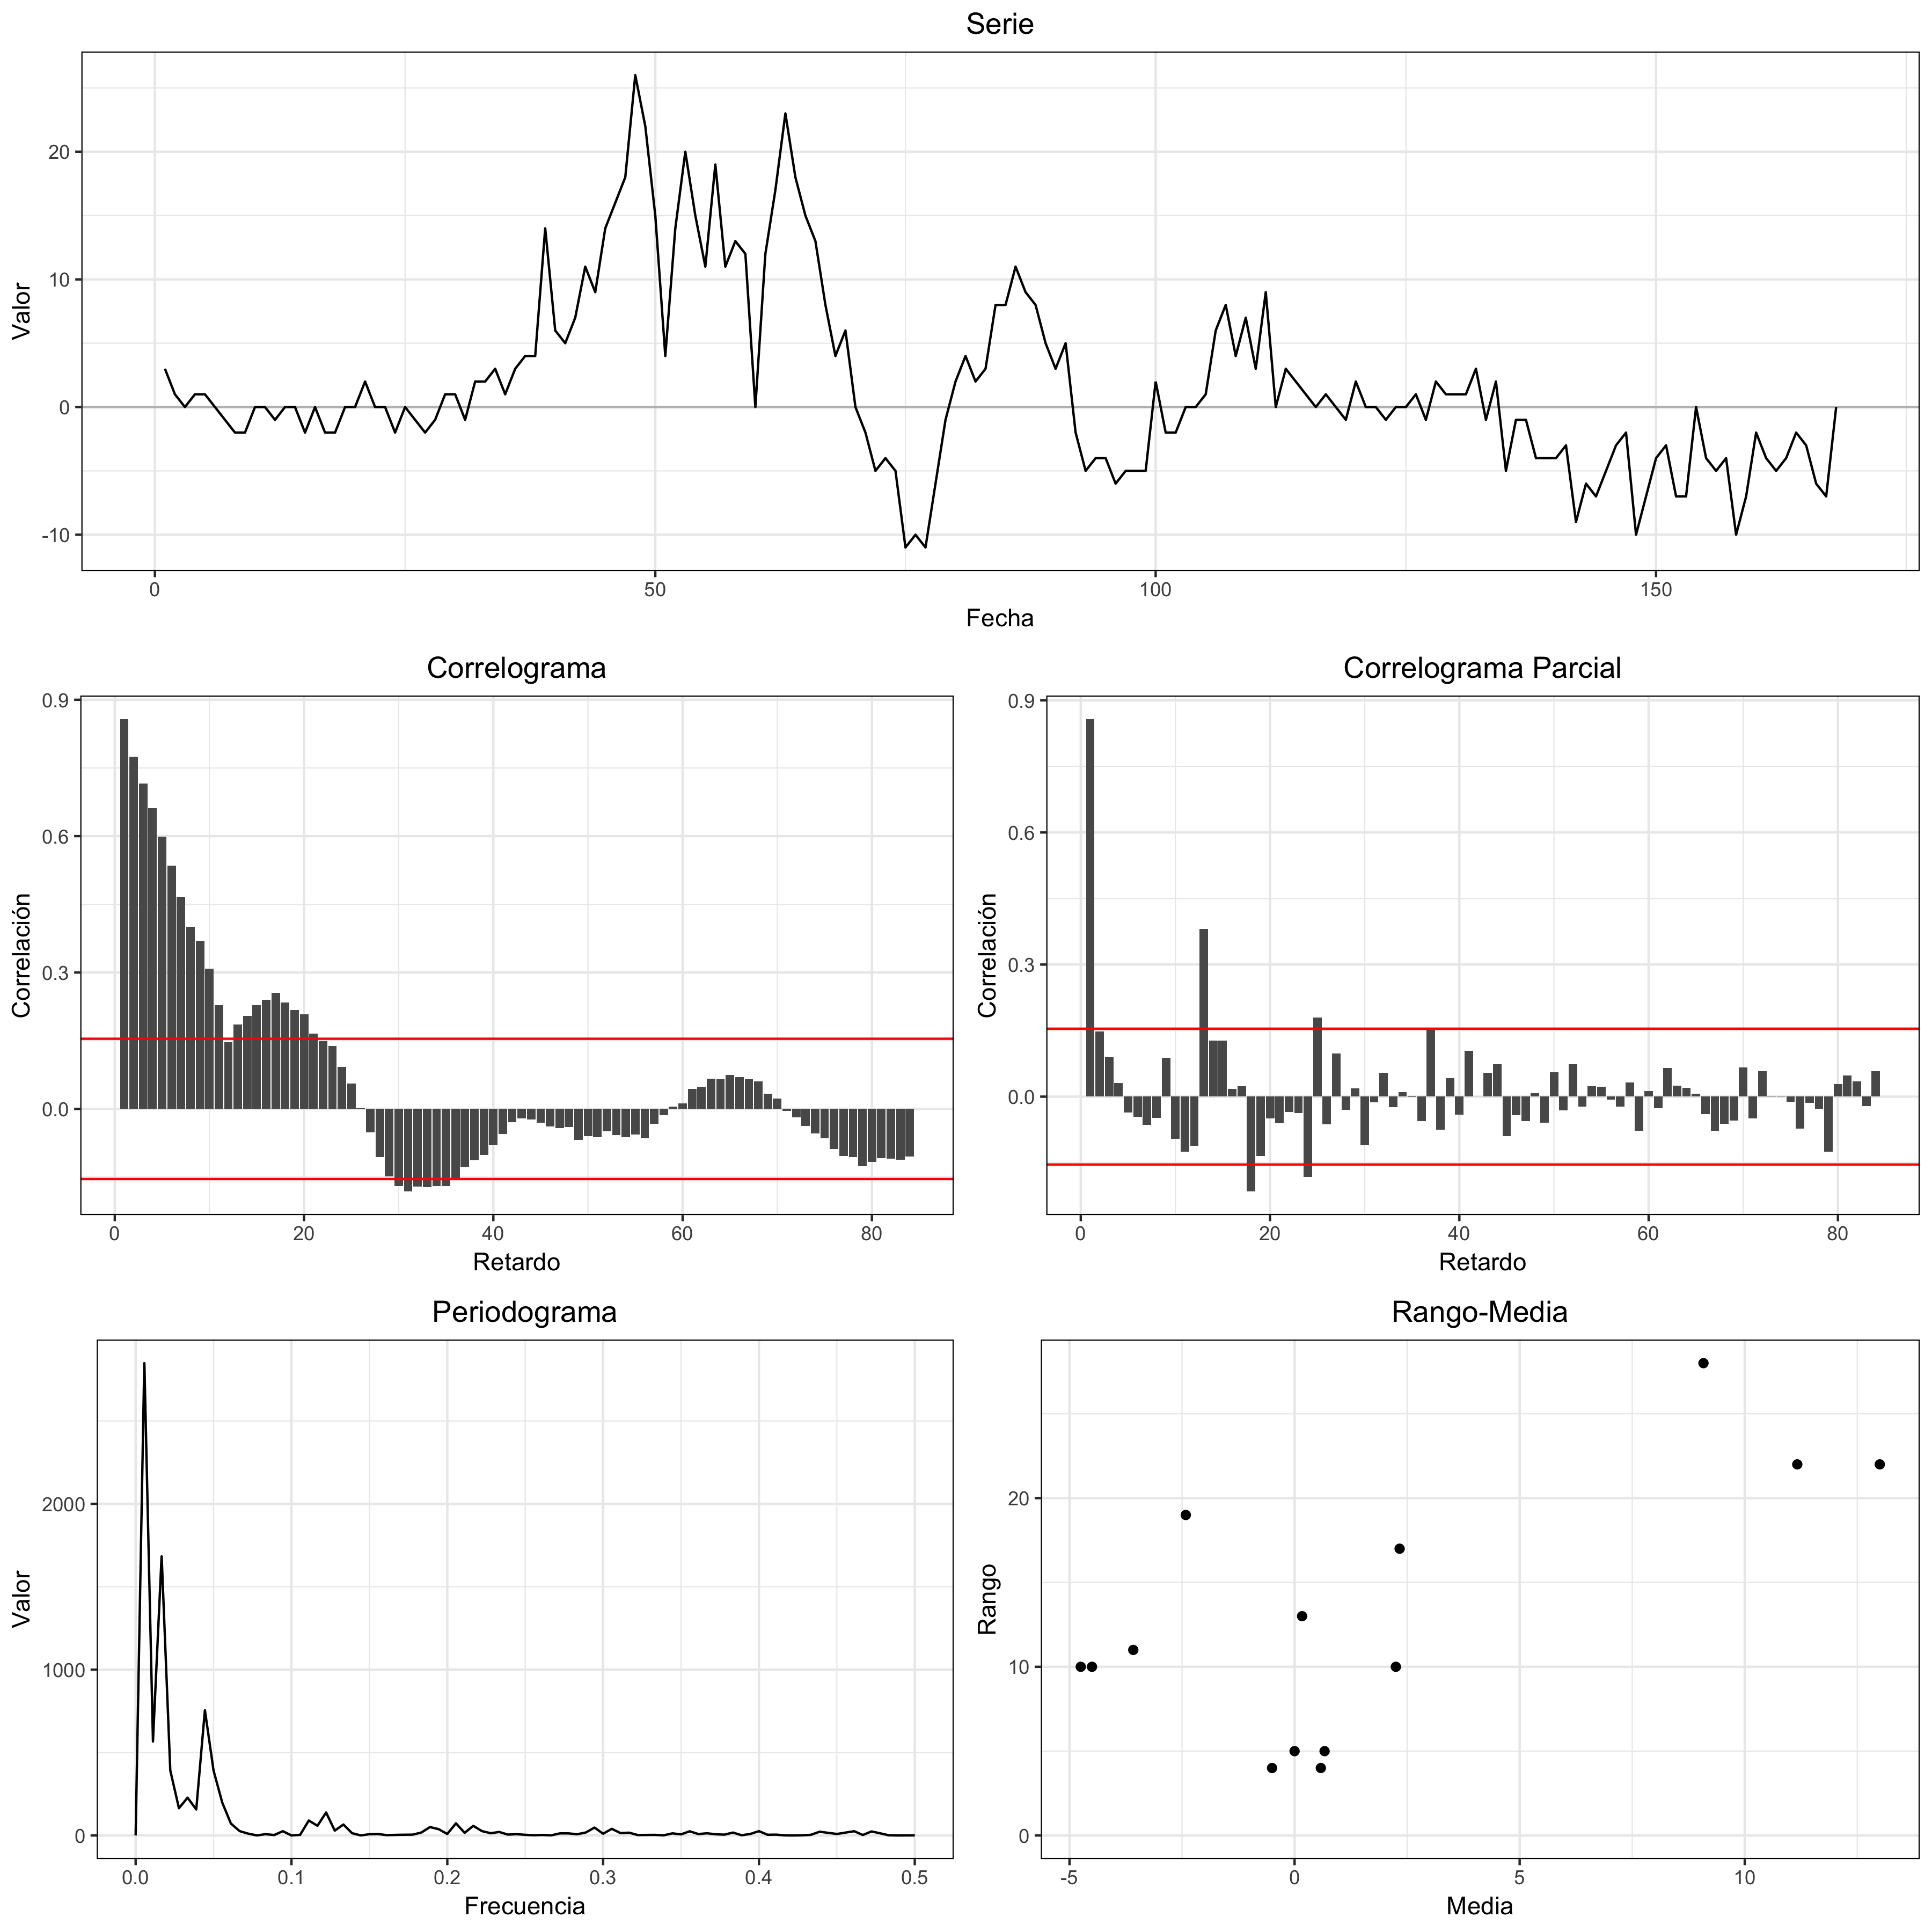
\includegraphics[width=\textwidth,height=\textheight,keepaspectratio]{weightloss-diff-12}
          \caption{Gráfico de la serie, Correlograma, Correlograma Parcial, Periodograma y diagrama de dispersión \emph{rango-media} para la serie \texttt{weightloss} tras la realización de una diferenciación estacional (12 retardos).}
          \label{img:weightloss_diff_12}
        \end{figure}

        \paragraph{}
        En el gráfico de la serie se puede apreciar la eliminación de la estructura estacional tras la serie, pero no la tendencia de la misma. Ahora la serie obscila en torno a valores próximos a cero, pero la tendencia hace que este comportamiento no pueda ser considerado estacionario. En el correlograma sucede algo similar: en este caso se ha conseguido eliminar la estructura lineal de decrecimientos en las correlaciones de la estacionalidad, pudiéndose considerar ahora decrecimiento exponencial. Sin embargo, la componente regular no tiene una estructura de decrecimientos exponenciales, lo cual hacer rechazar la hipótesis de que la serie sea estacionaria. En cuanto al correlograma parcial, se puede apreciar que se han reducido drásticamente las correlaciones referidas a los múltiplos de la estacionalidad, pero siguen destacando en gran medida las correlaciones en las posiciones 1 y 13. Se cree que la primera correlación se debe a la componente de tendencia de la seria, siendo la del 13-ésimo retardo un reflejo estacional de esta. En cuanto al periodograma, se puede apreciar que el primer armónico destaca en gran medida sobre el resto, lo cual se cree que es debido a la tendencia de la serie. En cuanto al diagrama de dispersión \emph{rango-media}, se puede ver que la relación entre nivel y dispersión ha aumentado, lo cual es otro reflejo de que la serie resultante no es estacionaria.


        \paragraph{}
        La diferenciación estacional ha conseguido reducir en gran medida la componente estacional de la serie. En la \autoref{table:variance_differences} se indica que la la varianza es $49.09$, lo cual es una drástica reducción en la dispersión de la serie. Sin embargo ha dejado inalterada la tendencia de la misma, por lo que no se ha conseguido llegar a una serie estacionaria, que tomar de partida para el ajuste de un modelo autoregresivo con media móvil. Como se verá a continuación, la serie se transforma en estacionaria tras aplicar una combinación de las dos diferenciaciones realizadas previamente. Esto es, la diferenciación regular y la diferenciación regular, que aisla tanto la tendencia de la serie, como la estructura estacional de la misma.

      \subsubsection{Diferenciación regular y estacional}
      \label{sec:regular_seasonal_difference}

        \paragraph{}
        Tras analizar los resutados obtenidos al aplicar la diferenciación regular y la diferenciación estacional, para la cual se producen distintas modificaciones de la serie original que la dejan más cerca de la propiedad de estacionaridad, el siguiente paso es combinar ambas estrategias. Dado que la operación de diferenciación es conmutativa, no importa el orden de aplicación. En este caso, se ha desarrollado la expresión conjunta en la \autoref{eq:diff_1_12}.

        \begin{equation}
        \label{eq:diff_1_12}
          \begin{split}
            \nabla \nabla_{12} X_t
            &= (1 - B) \cdot (1 - B^{12}) \cdot X_t \\
            &= (1 - B) \cdot (X_t - X_{t - 12}) \\
            &= X_t - X_{t - 1} - X_{t - 12} + X_{t - 13}
          \end{split}
        \end{equation}

        \paragraph{}
        En la \autoref{img:weightloss_diff_1_12} se muestran distintos resúmenes visuales de la serie diferenciada regular y estacionalmente. En el gráfico de la serie se observa como la tendencia de la serie ha sido eliminada, al igual que la estacionalidad, lo cual hace que el comportamiento de la serie sea mucho más similar a un ruido blanco, aunque sin llegar a serlo, tal y como se puede apreciar a partir del resto de gráficos. Llama la atención el aumento de la dispersión en torno al primer cuarto de la serie, lo cual asumimos que podría deverse al cambio de nivel durante finales del año $2008$ en la serie original. En cuanto al correlograma, se puede apreciar un decrecimiento exponencial en las primeras correlaciones. De la misma manera, tambien se puede apreciar un decrecimiento exponencial en las correlaciones estacionales. Estas son las de la forma $12i$, es decir, las correlacioens múltiplo de 12. Dichos decrecimientos exponenciales son un indicador de que la serie resultante será estacionaria. Sobre el correlograma parcial, en este caso también se muestran decrecimientos exponenciales. Sin embargo, tanto este fenómeno como un análisis más detallado del correlograma, serán llevados a cabo en la \autoref{sec:proposed_models} cuando se propongan distintos modelos \emph{SARIMA}. En el periodograma se puede apreciar como destacan de una serie de armónicos sobre el resto. Sin embargo, en este caso no lo hacen de manera determinista, por lo que no pueden ser considerados una única estacionalidad que poder aislar de manera sencilla. Por lo tanto, lo trataremos como una componente aleatoria. Por último, a través del diagrama de dispersión \emph{rango-media} se puede comprobar que la relación entre nivel y dispersión ha desaparecido. Entonces, ya podemos considerar que la serie resultante cumple la propiedad de \emph{homocedastecidad}.

        \begin{figure}[htb!]
          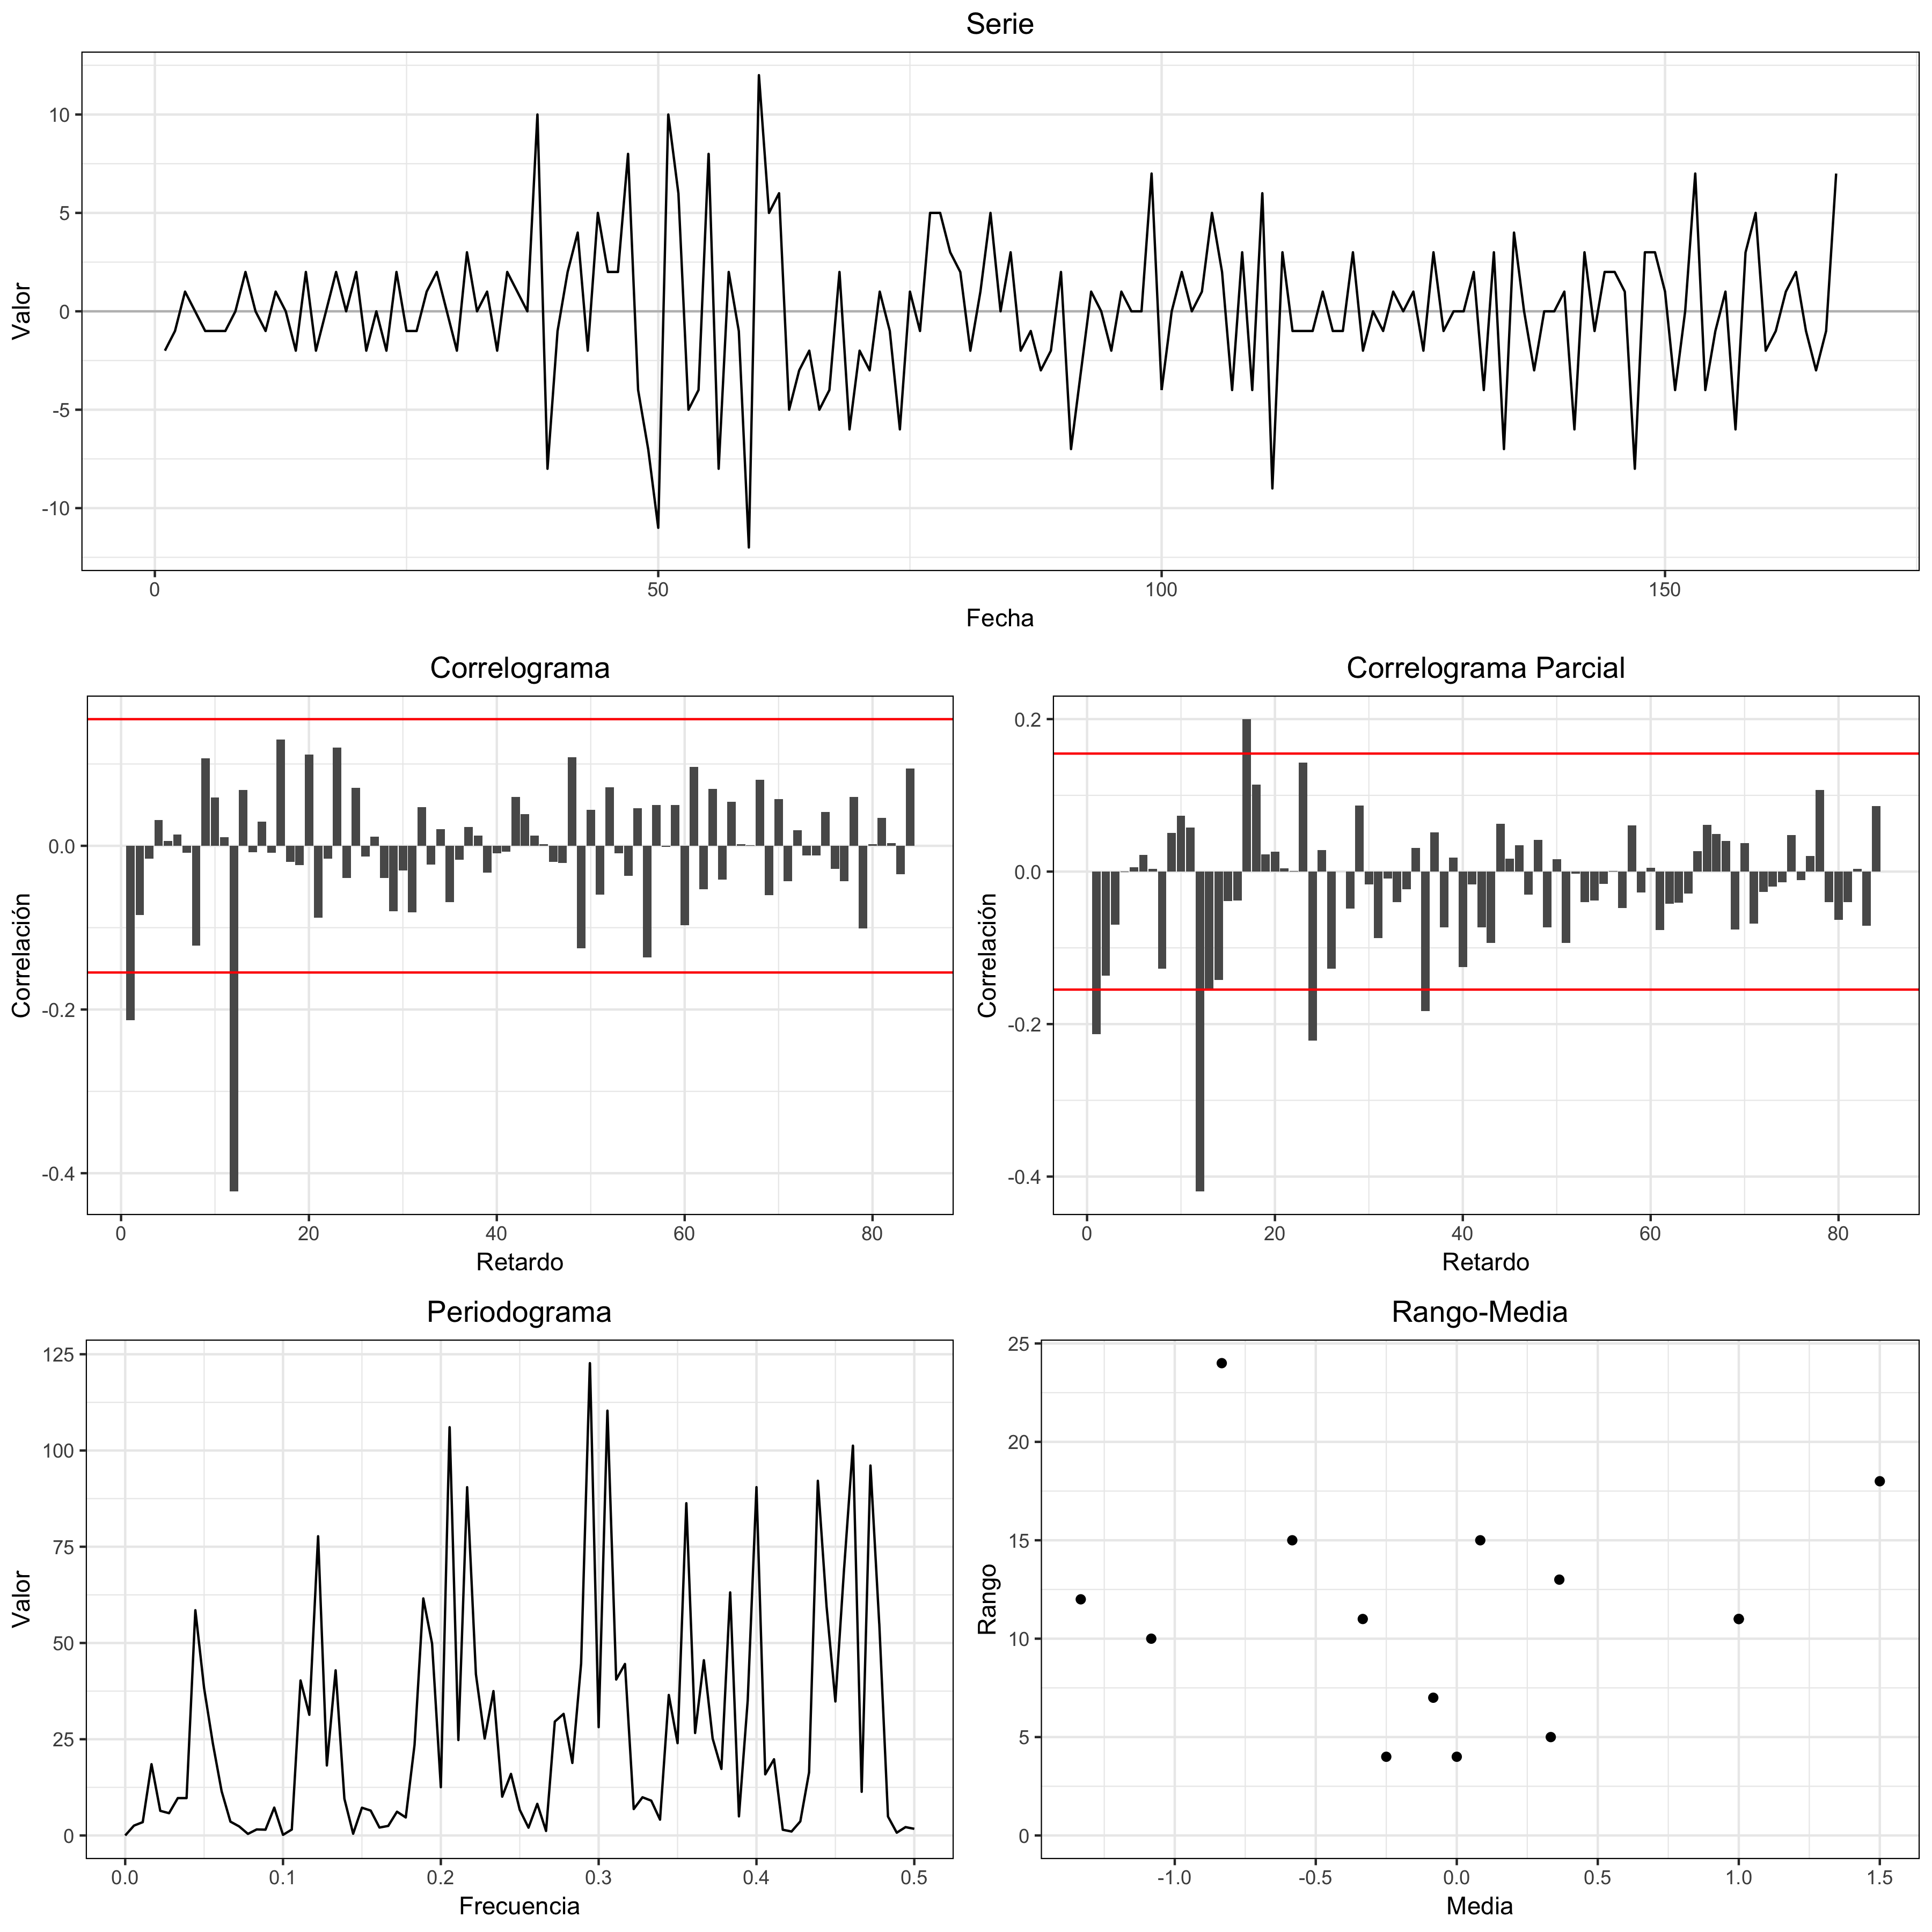
\includegraphics[width=\textwidth,height=\textheight,keepaspectratio]{weightloss-diff-1-12}
          \caption{Gráfico de la serie, Correlograma, Correlograma Parcial, Periodograma y diagrama de dispersión \emph{rango-media} para la serie \texttt{weightloss} tras la realización de una diferenciación regular y otra diferención estacional (12 retardos).}
          \label{img:weightloss_diff_1_12}
        \end{figure}

        \paragraph{}
        Dado que la serie cumple la propiedad de media y varianza constantes a lo largo del tiempo y además presenta decrecimientos exponenciales en el correlograma, consideraremos que la serie resultante es estacionaria. Además, la varianza de $14.07$ es la menor que se ha obtenido, tal y como se puede apreciar en la \autoref{table:variance_differences}. Por estas razones, diremos que una diferenciación regular y otra estacional son suficientes para conseguir la propiedad de estacionaridad, necesaria para el ajuste de un modelo \emph{SARIMA}.

        \paragraph{}
        Por último, se desea comprobar si la media de la serie puede ser considerada significativamente distinta de $0$, en cuyo caso deberíamos ajustar un modelo con término independiente. Para ello, se ha llevado a cabo un test \emph{t de student}, tras el cual se ha obtenido un valor $t_{obs} = -0.061898$ lo cual indica el $pvalor = 0.9507$, no teniendo evidencias para el rechazo. Dicho test se incluye en el \autoref{code:descriptive_r}. Además, a continuación se incluye el resultado de dicho test:

        \begin{figure}
          \begin{Verbatim}
            One Sample t-test
            t = -0.061898, df = 166, p-value = 0.9507
            alternative hypothesis: true mean is not equal to 0
            95 percent confidence interval:
             -0.5909606  0.5550325
            sample estimates:
              mean of x
            -0.01796407
          \end{Verbatim}
          \caption{Resultados del test \emph{t de student} sobre la media nula ($H_0: \mu = 0$) para la serie \emph{weightloss} diferenciada regular y estacionalmente.}
          \label{result:zero_mean_test}
        \end{figure}

    \paragraph{}
    Una vez realizado el análisis descriptivo de la serie, así como la búsqueda por los órdenes de diferenciación necesarios para conseguir estacionarizar nuestra serie, ya estamos en condiciones de analizar la serie desde otro punto de vista: la proposición de modelos, lo cual se expone a continuación.

    \subsection{Modelos propuestos}
    \label{sec:proposed_models}

      \paragraph{}
      Tal y como se ha dicho posteriormente, en este apartado se van a proponer distintos modelos para el ajuste de la serie. Estos se proponen teniendo en cuenta únicamente el análisis descriptivo de la serie original, así como de las diferenciadas. Puesto que ya se ha decidido el grado de diferenciacion de la serie en la \autoref{sec:seasonal_difference} este será un valor fijo en la proposición de modelos. Esto se debe a que el ajuste de este tipo de modelos requiere de la estacionarización de la serie original.

      \paragraph{}
      Para indicar los modelos se utilizará la notación que se describe en la \autoref{eq:sarima}, donde la primera tupla se refiere a los parámetros regulares, mientras que las subsiguientes se refieren al periodo estacional $s_i$-ésimo en cada caso. El parámetro $p$ indica el orden de la componente autoregresiva en cada tupla, el parámetro $d$ se refiere al grado de diferenciación y por último, el parámetro $q$ al orden de la componente de media móvil.

      \begin{equation}
      \label{eq:sarima}
        \text{SARIMA}(p, d, q)(P_1, D_1, Q_1)_{s_1}(P_2, D_2, Q_2)_{s_2}...(P_q, D_q, Q_q)_{s_q}
      \end{equation}

      \paragraph{}
      Puesto que anteriormente se indicó que era necesaria una diferenciación regular y otra estacional (de longitud $12$) en la \autoref{sec:regular_seasonal_difference}, sabemos que los modelos proputestos serán de la forma $\text{SARIMA}(p, 1, q)(P, 1, Q)_{12}...(P_q, D_q, Q_q)_{s_q}$. Para proponer modelos, nos vamos a fijar en la \autoref{img:weightloss_diff_1_12}, que recoge distintos gráficos sobre la serie diferenciada regular y estacionalmente. En concreto, nos fijaremos sobre todo tanto en el correlograma como en el correlograma parcial, el cual sirve de guía a la hora de elegir órdenes de las componentes autorregresivas y de medias móviles.

      \paragraph{}
      El primer modelo que se propone es el indicado en la \autoref{eq:sarima_1}, el cual se basa en la utilización de $1$ parámetro de media móvil en la parte regular y otro en la parte estacional de periodicidad $12$. La justificación detrás de este modelo es la siguiente: se pueden apreciar decrecimientos exponenciales en el diagrama de correlación parcial que comienzan en los retardos $1$ y $12$. Además, se dan valores elevados en el correlograma en las correlaciones $1$ y $12$, lo cual es implica que un modelo de esta forma podría ajustarse de manera coherente a la serie.

      \begin{equation}
        \label{eq:sarima_1}
        \text{SARIMA}(0, 1, 1)(0, 1, 1)_{12}
      \end{equation}

      \paragraph{}
      Se intuye que el modelo de la \autoref{eq:sarima_1} será el más adecuado para la serie \texttt{weightloss}. Sin embargo, a continuación se proponen otros modelos para los que se cree que existen distintas razones por las cuales se deberían comportar de manera adecuada.

      \paragraph{}
      El modelo de la \autoref{eq:sarima_2} consiste en una ampliación respecto del anterior. En este se ha añadido $1$ parámetro de media móvil más, en el retardo $17$. La razón por la cual se propone este modelo es el decrecimiento exponencial en el correlograma parcial de la \autoref{img:weightloss_diff_1_12}, que comienza en dicho retardo.

      \begin{equation}
        \label{eq:sarima_2}
        \text{SARIMA}(0, 1, 1)(0, 1, 1)_{12}(0, 0, 1)_{17}
      \end{equation}

      \paragraph{}
      Para completar la proposición de modelos que podrían ajustarse de manera adecuada a la serie, se añaden los indicados en la \autoref{eq:sarima_3} y en la \autoref{eq:sarima_4}, los cuales son ampliaciones de los indicados en la \autoref{eq:sarima_1} y en la \autoref{eq:sarima_2} respectivamente. Estos añaden $1$ parámetro autoregresivo a la componente regular de la serie. La justificación sobre este parámetro se debe al decrecimiento exponencial a partir del segundo retardo en el correlograma (ya que el valor del primer retardo proviene de la componente de media móvil). Si estos modelos finalmente son considerados válidos, entonces también habrá que considerar la primera correlación parcial como procedente de la componente autoregresiva regular. Sin embargo, se intuye que estos modelos finalmente será invalidados.

      \begin{equation}
        \label{eq:sarima_3}
        \text{SARIMA}(1, 1, 1)(0, 1, 1)_{12}
      \end{equation}

      \begin{equation}
        \label{eq:sarima_4}
        \text{SARIMA}(1, 1, 1)(0, 1, 1)_{12}(0, 0, 1)_{17}
      \end{equation}

      \paragraph{}
      El siguiente paso es proceder al ajuste de los modelos propuestos, prestando especial atención a la significancia de los tests para los parámetros en cada modelo, así como a los residuos obtenidos, los cuales permitirán validar (e invalidar) aquellos modelos que no se ajusten de manera satisfactoria a los datos.


  \section{Etapa de estimación y validación}
  \label{sec:fitting}

    \paragraph{}
    Una vez propuestos distintos modelos que podrían ajustar de manera adecuada a la serie, a continuación se procederá al ajuste de los mismos, para ello se utilizará el lenguaje \emph{SAS}.


    \subsection{Estimación y Validación de \textbf{$\text{SARIMA}(0, 1, 1)(0, 1, 1)_{12}$}}
    \label{sec:fitting_1}

      \paragraph{}
      [TODO]

      \begin{table}[htb!]
        \centering
        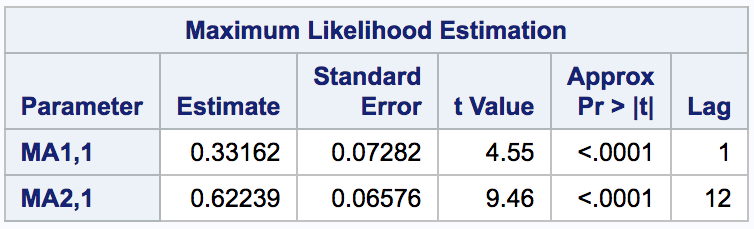
\includegraphics[width=0.6\textwidth]{validation-1-estimation}
        \caption{[TODO].}
        \label{}
      \end{table}

      \paragraph{}
      [TODO]

      \begin{table}[htb!]
        \centering
        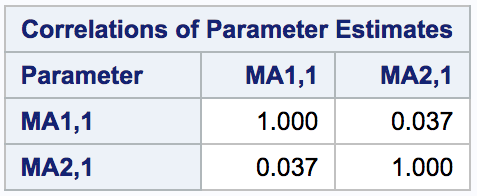
\includegraphics[width=0.4\textwidth]{validation-1-correlations}
        \caption{[TODO].}
        \label{}
      \end{table}

      \paragraph{}
      [TODO]

      \begin{table}[htb!]
        \centering
        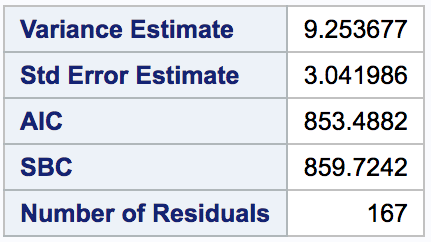
\includegraphics[width=0.3\textwidth]{validation-1-metrics}
        \caption{[TODO].}
        \label{}
      \end{table}

      \paragraph{}
      [TODO]

      \begin{table}[htb!]
        \centering
        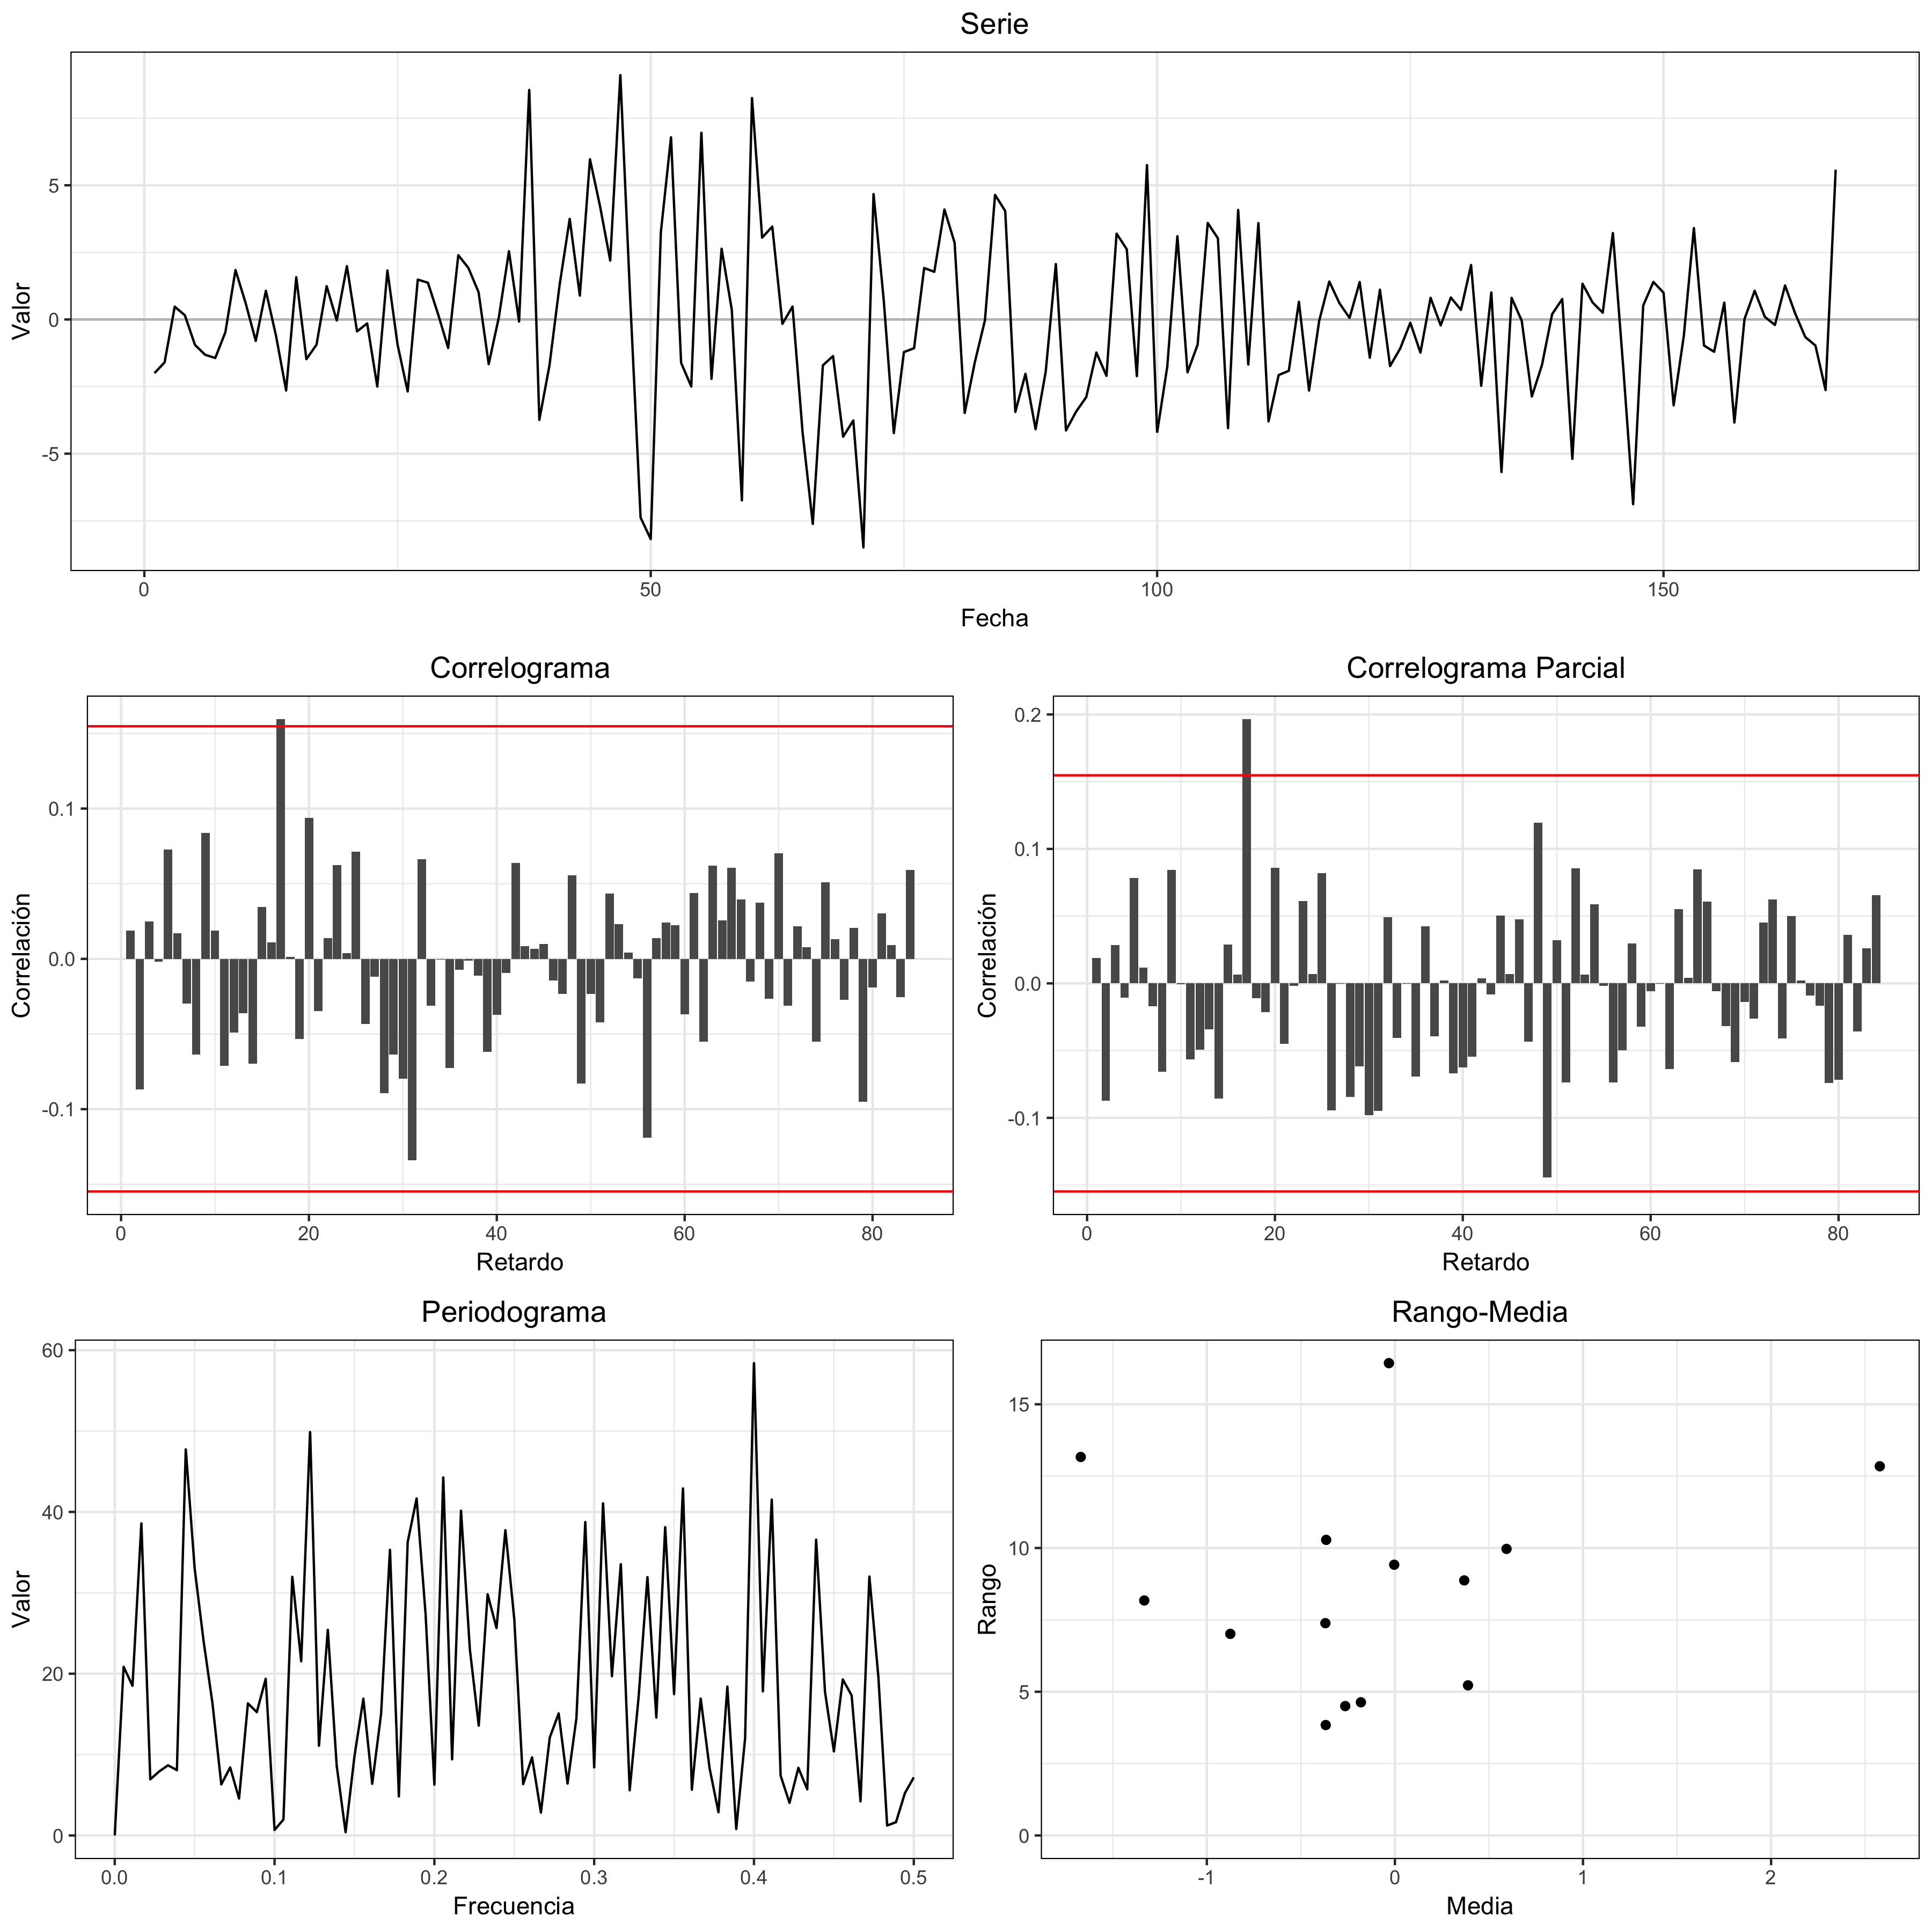
\includegraphics[width=\textwidth]{validation-1-residuals}
        \caption{[TODO].}
        \label{}
      \end{table}

      \paragraph{}
      [TODO]

      \begin{figure}
        \begin{Verbatim}
          Box-Ljung test
          X-squared = 0.059792, lag = 1, p-value = 0.8068
        \end{Verbatim}
        \caption{Resultados del test de \emph{Ljung-Box} de dependencia serial en los residuales ajustados por el modelo $\text{SARIMA}(0, 1, 1)(0, 1, 1)_{12}$}
        \label{result:comparison_1_ljung_box_1}
      \end{figure}

      \paragraph{}
      [TODO]

      \begin{figure}
        \begin{Verbatim}
          Box-Ljung test
          X-squared = 5.9799, lag = 12, p-value = 0.9171
        \end{Verbatim}
        \caption{Resultados del test de \emph{Ljung-Box} de dependencia estacional en los residuales ajustados por el modelo $\text{SARIMA}(0, 1, 1)(0, 1, 1)_{12}$}
        \label{result:comparison_1_ljung_box_12}
      \end{figure}

      \paragraph{}
      [TODO]

      \begin{table}[htb!]
        \centering
        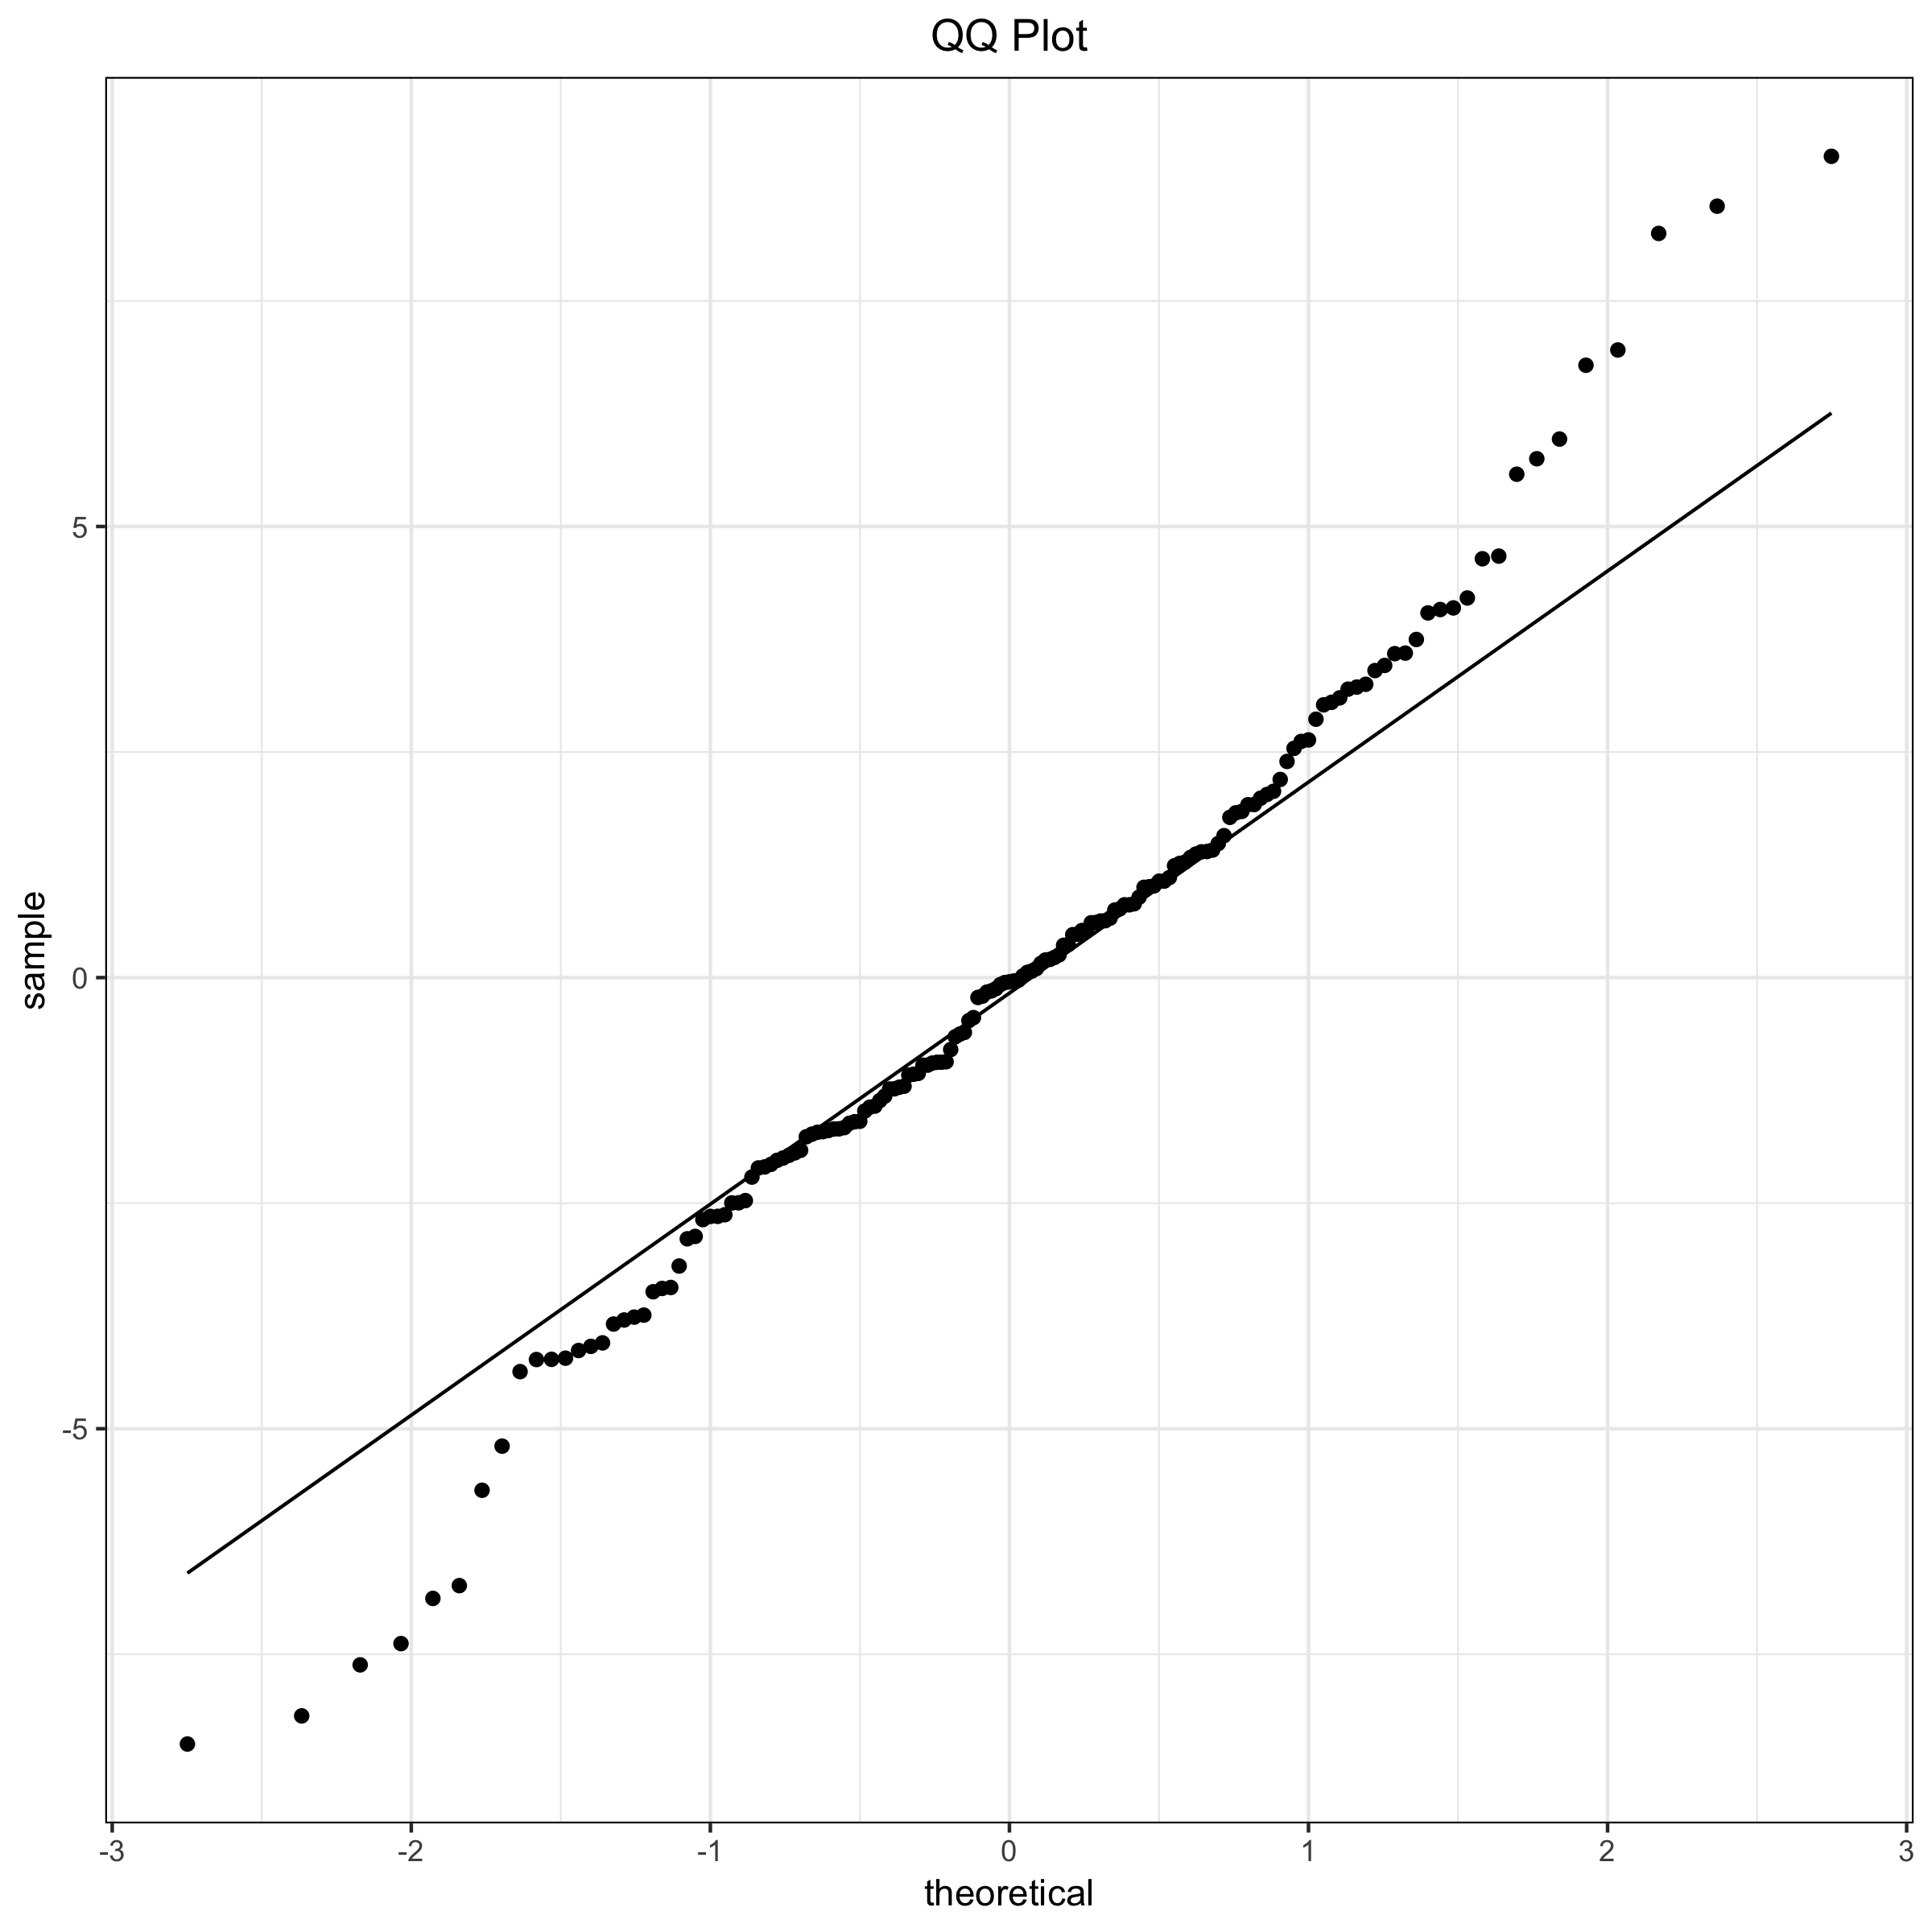
\includegraphics[width=0.7\textwidth]{validation-1-normality}
        \caption{[TODO].}
        \label{}
      \end{table}

      \paragraph{}
      [TODO]

      \begin{figure}
        \begin{Verbatim}
          Lilliefors (Kolmogorov-Smirnov) normality test
          D = 0.062944, p-value = 0.109
        \end{Verbatim}
        \caption{Resultados del test de \emph{Lilliefors} de normalidad en los residuales ajustados por el modelo $\text{SARIMA}(0, 1, 1)(0, 1, 1)_{12}$}
        \label{result:comparison_1_lilliefors}
      \end{figure}

      \paragraph{}
      [TODO]

      \begin{figure}
        \begin{Verbatim}
          Shapiro-Francia normality test
          W = 0.98217, p-value = 0.03111
        \end{Verbatim}
        \caption{Resultados del test de \emph{Shapiro-Francia} de normalidad en los residuales ajustados por el modelo $\text{SARIMA}(0, 1, 1)(0, 1, 1)_{12}$}
        \label{result:comparison_1_sf}
      \end{figure}

      \paragraph{}
      [TODO]

    \subsection{Estimación y Validación de \textbf{$\text{SARIMA}(0, 1, 1)(0, 1, 1)_{12}(0, 0, 1)_{17}$}}
    \label{sec:fitting_2}

      \paragraph{}
      [TODO]

      \begin{table}[htb!]
        \centering
        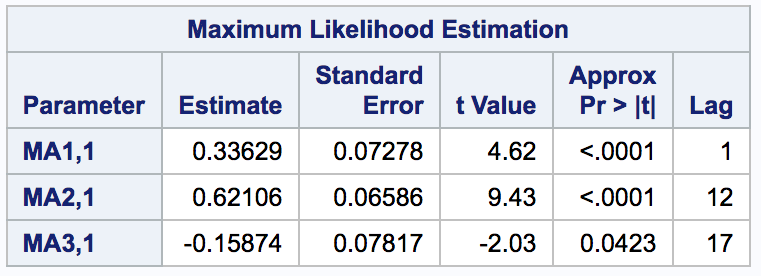
\includegraphics[width=0.6\textwidth]{validation-2-estimation}
        \caption{[TODO].}
        \label{}
      \end{table}

      \paragraph{}
      [TODO]

      \begin{table}[htb!]
        \centering
        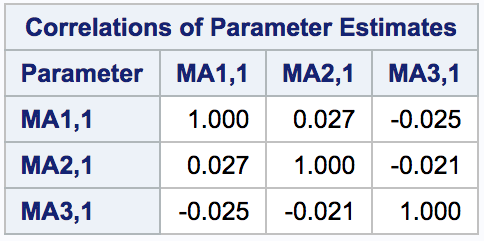
\includegraphics[width=0.4\textwidth]{validation-2-correlations}
        \caption{[TODO].}
        \label{}
      \end{table}

      \paragraph{}
      [TODO]

      \begin{table}[htb!]
        \centering
        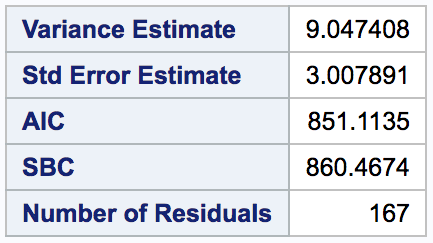
\includegraphics[width=0.3\textwidth]{validation-2-metrics}
        \caption{[TODO].}
        \label{}
      \end{table}

      \paragraph{}
      [TODO]

      \begin{table}[htb!]
        \centering
        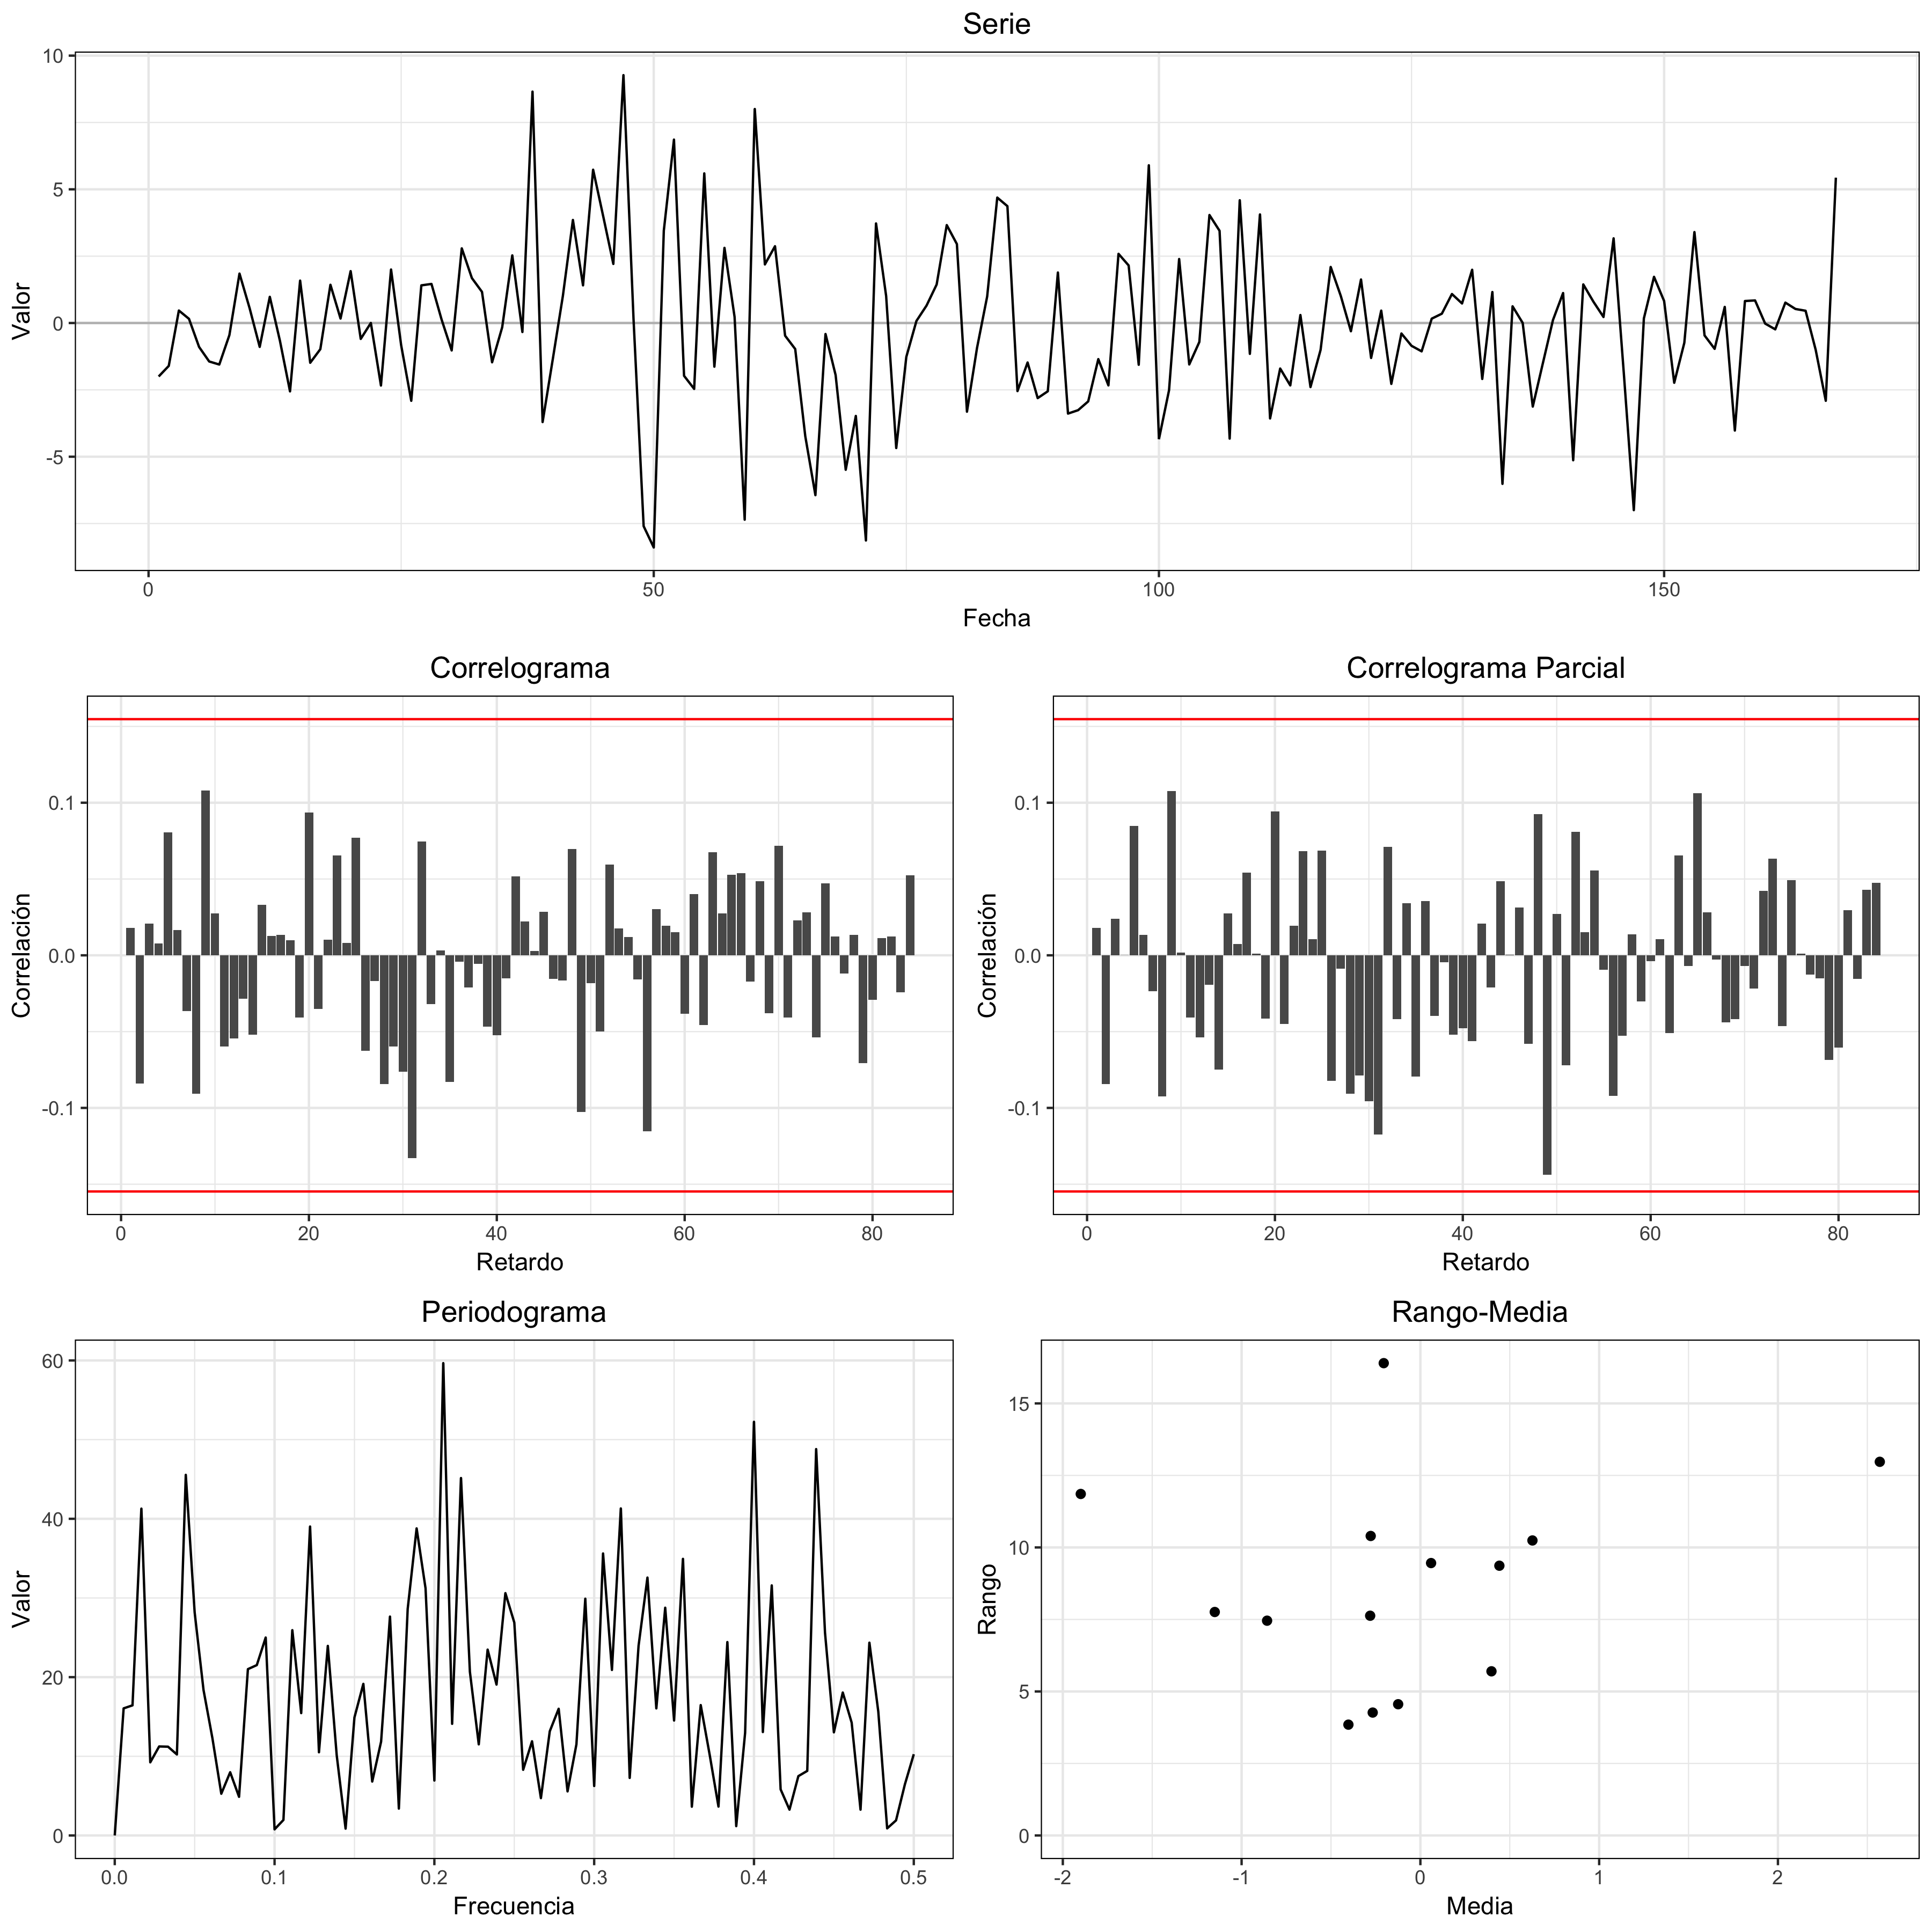
\includegraphics[width=\textwidth]{validation-2-residuals}
        \caption{[TODO].}
        \label{}
      \end{table}

      \paragraph{}
      [TODO]

      \begin{figure}
        \begin{Verbatim}
          Box-Ljung test
          X-squared = 0.055242, lag = 1, p-value = 0.8142
        \end{Verbatim}
        \caption{Resultados del test de \emph{Ljung-Box} de dependencia serial en los residuales ajustados por el modelo $\text{SARIMA}(0, 1, 1)(0, 1, 1)_{12}(0, 0, 1)_{17}$}
        \label{result:comparison_2_ljung_box_1}
      \end{figure}

      \paragraph{}
      [TODO]

      \begin{figure}
        \begin{Verbatim}
          Box-Ljung test
          X-squared = 7.6285, lag = 12, p-value = 0.8134
        \end{Verbatim}
        \caption{Resultados del test de \emph{Ljung-Box} de dependencia estacional en los residuales ajustados por el modelo $\text{SARIMA}(0, 1, 1)(0, 1, 1)_{12}(0, 0, 1)_{17}$}
        \label{result:comparison_2_ljung_box_12}
      \end{figure}

      \paragraph{}
      [TODO]

      \begin{table}[htb!]
        \centering
        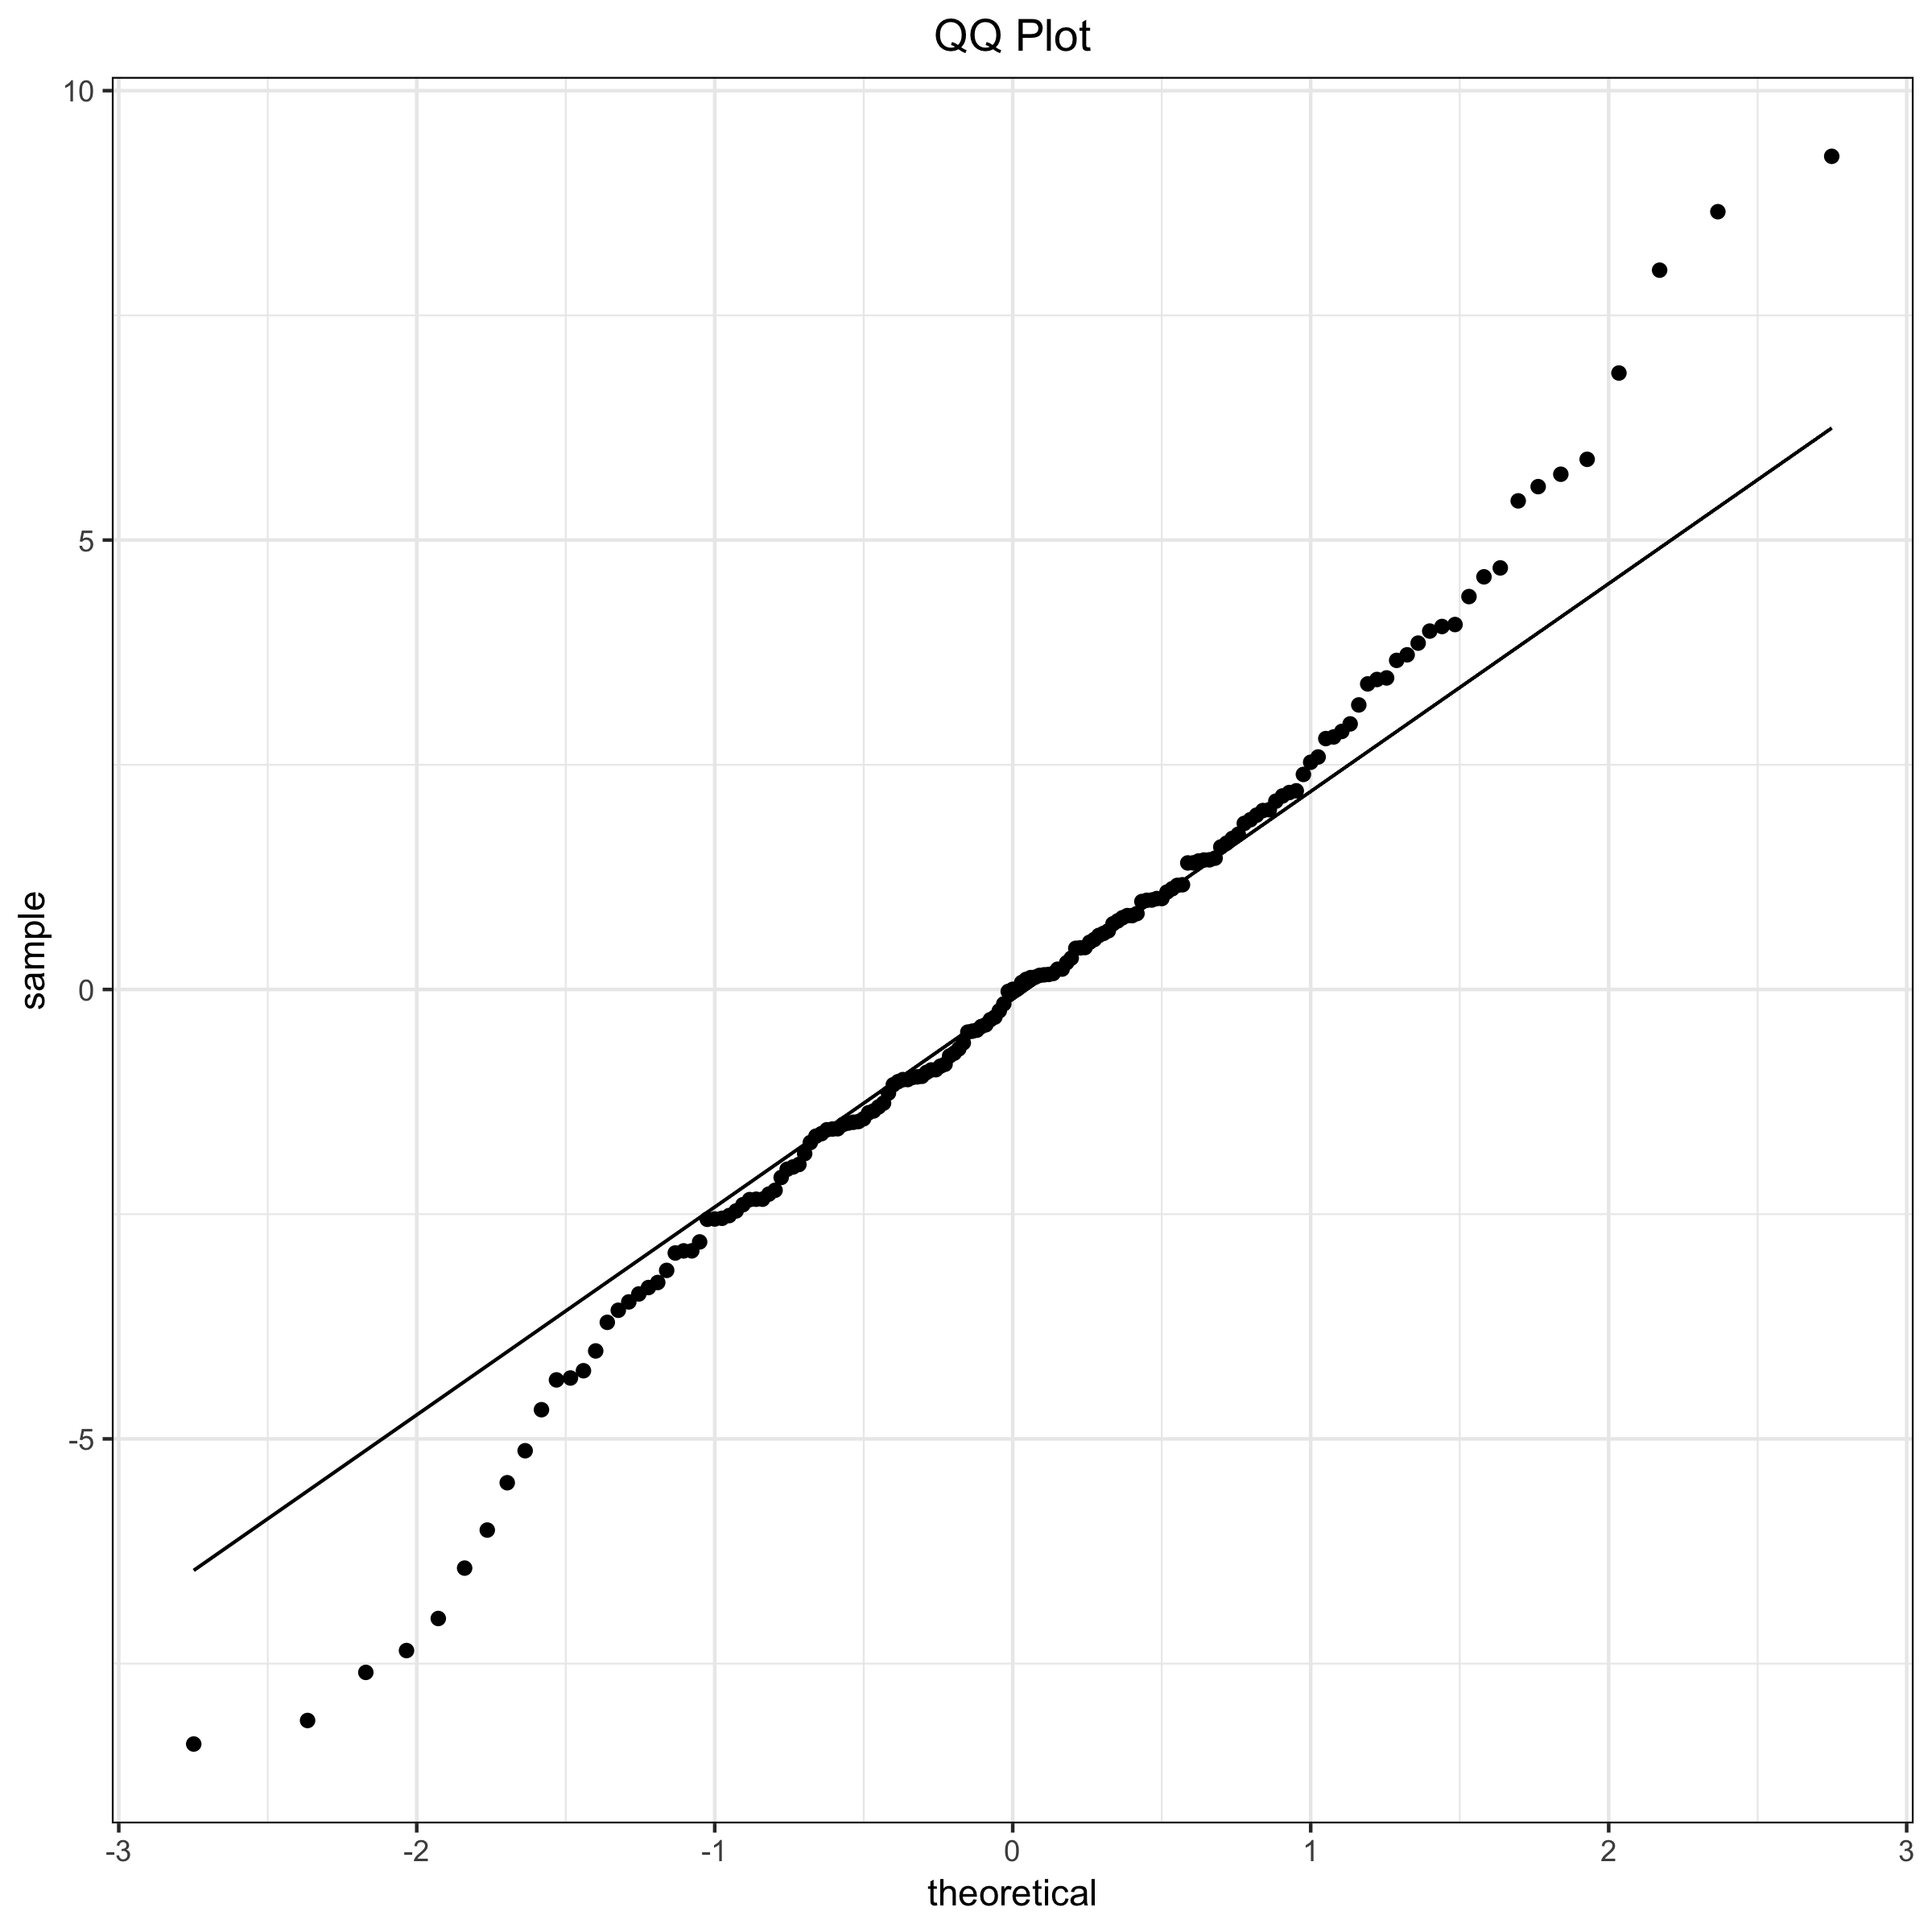
\includegraphics[width=0.7\textwidth]{validation-2-normality}
        \caption{[TODO].}
        \label{}
      \end{table}

      \paragraph{}
      [TODO]

      \begin{figure}
        \begin{Verbatim}
          Lilliefors (Kolmogorov-Smirnov) normality test
          D = 0.056905, p-value = 0.2067
        \end{Verbatim}
        \caption{Resultados del test de \emph{Lilliefors} de normalidad en los residuales ajustados por el modelo $\text{SARIMA}(0, 1, 1)(0, 1, 1)_{12}(0, 0, 1)_{17}$}
        \label{result:comparison_2_lilliefors}
      \end{figure}

      \paragraph{}
      [TODO]

      \begin{figure}
        \begin{Verbatim}
          Shapiro-Francia normality test
          W = 0.98119, p-value = 0.02422
        \end{Verbatim}
        \caption{Resultados del test de \emph{Shapiro-Francia} de normalidad en los residuales ajustados por el modelo $\text{SARIMA}(0, 1, 1)(0, 1, 1)_{12}(0, 0, 1)_{17}$}
        \label{result:comparison_2_sf}
      \end{figure}

      \paragraph{}
      [TODO]

    \subsection{Estimación y Validación de \textbf{$\text{SARIMA}(1, 1, 1)(0, 1, 1)_{12}$}}
    \label{sec:fitting_3}

      \paragraph{}
      [TODO]

      \begin{table}[htb!]
        \centering
        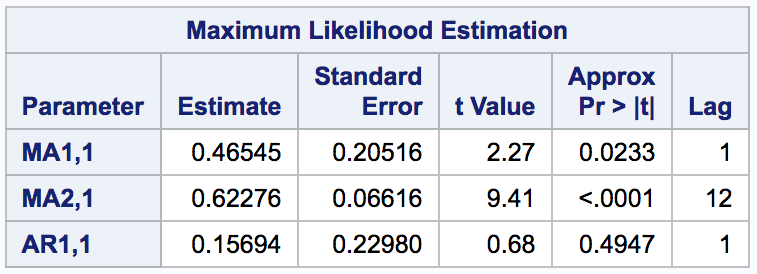
\includegraphics[width=0.6\textwidth]{validation-3-estimation}
        \caption{[TODO].}
        \label{}
      \end{table}

      \paragraph{}
      [TODO]

      \begin{table}[htb!]
        \centering
        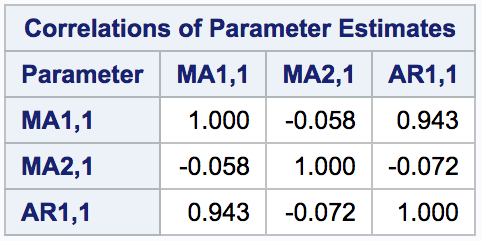
\includegraphics[width=0.4\textwidth]{validation-3-correlations}
        \caption{[TODO].}
        \label{}
      \end{table}

      \paragraph{}
      [TODO]

      \begin{table}[htb!]
        \centering
        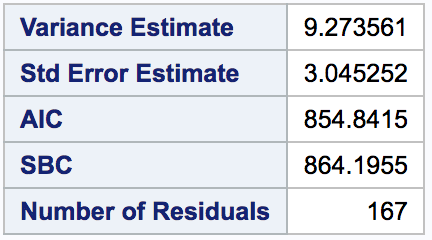
\includegraphics[width=0.3\textwidth]{validation-3-metrics}
        \caption{[TODO].}
        \label{}
      \end{table}

      \paragraph{}
      [TODO]

    \subsection{Estimación y Validación de $\textbf{SARIMA}(1, 1, 1)(0, 1, 1)_{12}(0, 0, 1)_{17}$}
    \label{sec:fitting_4}

      \paragraph{}
      [TODO]

      \begin{table}[htb!]
        \centering
        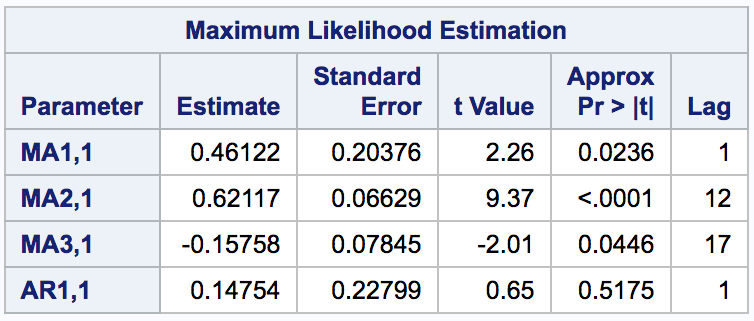
\includegraphics[width=0.6\textwidth]{validation-4-estimation}
        \caption{[TODO].}
        \label{}
      \end{table}

      \paragraph{}
      [TODO]

      \begin{table}[htb!]
        \centering
        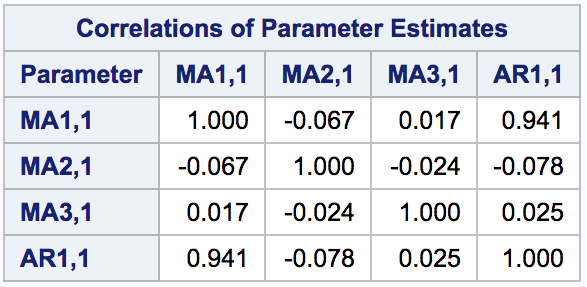
\includegraphics[width=0.4\textwidth]{validation-4-correlations}
        \caption{[TODO].}
        \label{}
      \end{table}

      \paragraph{}
      [TODO]

      \begin{table}[htb!]
        \centering
        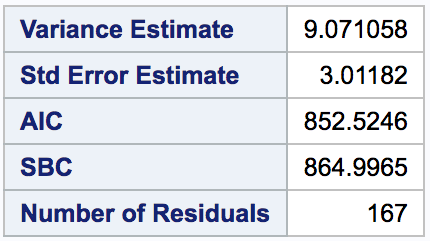
\includegraphics[width=0.3\textwidth]{validation-4-metrics}
        \caption{[TODO].}
        \label{}
      \end{table}

      \paragraph{}
      [TODO]


  \section{Comparación de modelos}
  \label{sec:comparison}
    \paragraph{}
    [TODO]


    \paragraph{}
    Para calcular el $SSE_p$, primero explicaremos resumidamente qué es así como en qué está basado. El $SSE_p$ es se corresponde con el cálculo de una medida para comparar la capacidad de predicción de un modelo de serie temporale. Se trata de predecir observaciones de una serie estacional de periodo $s$, para medir la capacidad de predicción de un modelo ajustado a dicha serie.

    \paragraph{}
    Si se dispone de $n$ observaciones en total, $x_1, x_2, ..., x_n$ se reservan las últimas $k$ observaciones, donde $k$ es un múltiplo de $s$. Para el ajuste se utilizan $m$ observaciones ($m = n - k$) y la medida se obtiene sumando los cuadrados de los residuales $\{1, 2, ..., k\}$ pasos hacia adelante. Esto se define en la \autoref{eq:sse_p}.

    \begin{equation}
    \label{eq:sse_p}
      \begin{split}
        SSE_p
        &= \sum_{j = 1} ^ k (x_{m + j} - x_{m}(j)) ^ 2 \\
        &= \sum_{j = 1} ^ k e_m(j) ^ 2 \\
        &= e_m(1) ^ 2 + e_m(2) ^ 2 + ... + e_m(k) ^ 2
      \end{split}
    \end{equation}

    \paragraph{}
    [TODO]

    \begin{table}[htb!]
      \centering
      \begin{tabular}{|l|r|r|r|r|r|r|}
          \hline
          \textbf{Fecha} & \textbf{Obs.} & \textbf{Predicho} & \textbf{Error Est.}& \textbf{L. Inf. ($95\%$)} & \textbf{L. Sup. ($95\%$)}  & \textbf{Residuo}
          \csvreader[
           head to column names,
          ]{res/data/comparison-1-reduced.csv}{}
          {\\ \hline \Month & \Weightloss & \FORECAST & \STD & \L & \U & \RESIDUAL}
          \\\hline
      \end{tabular}
      \caption{Predicción $12$ observaciones hacia delante, reservando las $12$ últimas para calcular el $SSE_p$ de la serie \texttt{weightloss} utilizando el modelo $\text{SARIMA}(0, 1, 1)(0, 1, 1)_{12}$.}
      \label{table:comparison-1}
    \end{table}

    \paragraph{}
    [TODO]

    \begin{table}[htb!]
      \centering
      \begin{tabular}{|l|r|r|r|r|r|r|}
          \hline
          \textbf{Fecha} & \textbf{Obs.} & \textbf{Predicho} & \textbf{Error Est.}& \textbf{L. Inf. ($95\%$)} & \textbf{L. Sup. ($95\%$)}  & \textbf{Residuo}
          \csvreader[
           head to column names,
          ]{res/data/comparison-2-reduced.csv}{}
          {\\ \hline \Month & \Weightloss & \FORECAST & \STD & \L & \U & \RESIDUAL}
          \\\hline
      \end{tabular}
      \caption{Predicción $12$ observaciones hacia delante, reservando las $12$ últimas para calcular el $SSE_p$ de la serie \texttt{weightloss} utilizando el modelo $\text{SARIMA}(0, 1, 1)(0, 1, 1)_{12}(0, 1, 1)_{17}$.}
      \label{table:comparison-2}
    \end{table}

    \paragraph{}
    [TODO]

    \begin{table}[htb!]
      \centering
      \begin{tabular}{|l|r|}
          \hline
          \textbf{Modelo} & \textbf{$SSE_p$}
          \csvreader[
            head to column names
          ]{res/data/predict-error.csv}{}
          {\\ \hline \name & \error}
          \\\hline
      \end{tabular}
      \caption{Suma de Cuadrados del Error de Predicción acumulada para $12$ observaciones hacia delante para los modelos $\text{SARIMA}(0, 1, 1)(0, 1, 1)_{12}$ y $\text{SARIMA}(0, 1, 1)(0, 1, 1)_{12}(0, 0, 1)_{17}$.}
      \label{table:sse_p}
    \end{table}

    \paragraph{}
    [TODO]

    \begin{figure}[htb!]
      \centering
      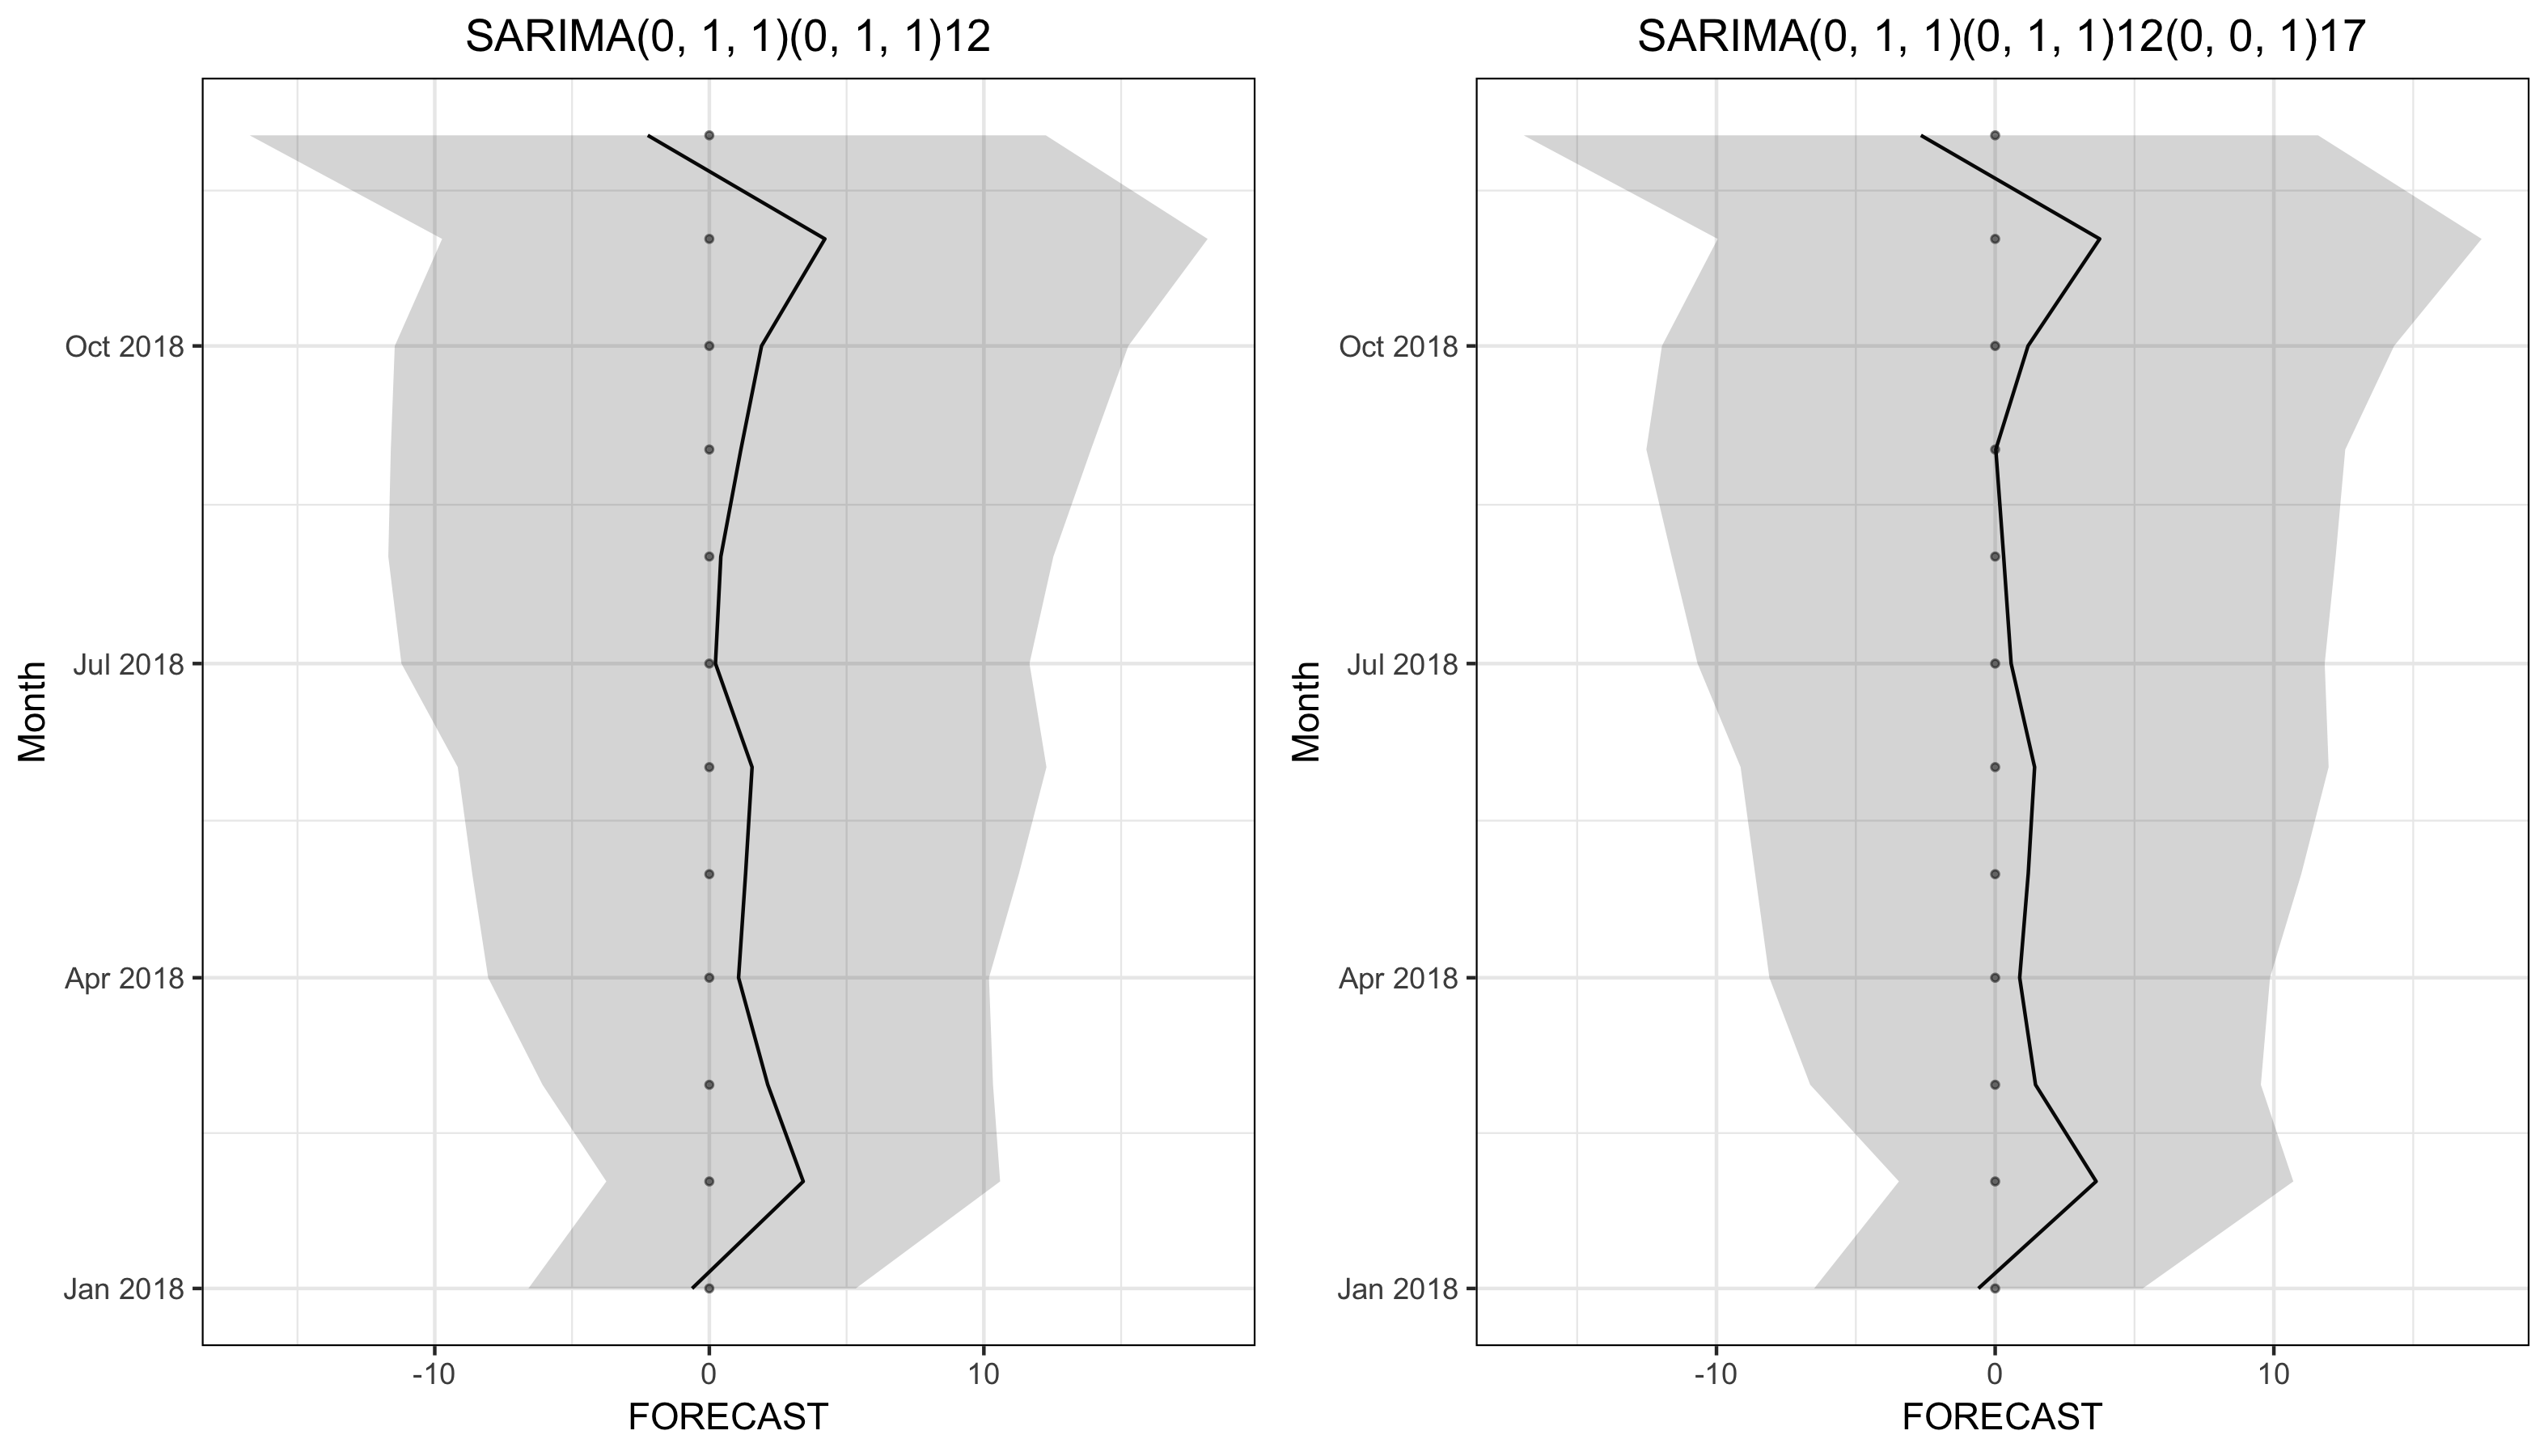
\includegraphics[width=\textwidth]{comparison-ci-amplitude}
      \caption{Comparación de las amplitudes de los intervalos de predicción para los modelos $\text{SARIMA}(0, 1, 1)(0, 1, 1)_{12}$ y $\text{SARIMA}(0, 1, 1)(0, 1, 1)_{12}(0, 0, 1)_{17}$.}
      \label{img:ci_amplitude}
    \end{figure}

    \paragraph{}
    [TODO]

    \begin{figure}
      \begin{Verbatim}
        One Sample t-test

        t = -0.061898, df = 166, p-value = 0.9507
        alternative hypothesis: true mean is not equal to 0
        95 percent confidence interval:
        -0.5909606  0.5550325
        sample estimates:
        mean of x
        -0.01796407
      \end{Verbatim}
      \caption{Resultados del test \emph{t de student} sobre la media nula ($H_0: \mu = 0$) para la diferencia entre amplitudes en los intervalos de predicción para los modelos $\text{SARIMA}(0, 1, 1)(0, 1, 1)_{12}$ y $\text{SARIMA}(0, 1, 1)(0, 1, 1)_{12}(0, 0, 1)_{17}$.}
      \label{result:comparison_ci_zero_mean}
    \end{figure}

    \paragraph{}
    [TODO]

  \section{Predicción}
  \label{sec:prediction}

    \paragraph{}
    [TODO]

    \paragraph{}
    [TODO]

    \begin{table}[htb!]
      \centering
      \begin{tabular}{|l|r|r|r|r|r|r|}
          \hline
          \textbf{Fecha} & \textbf{Obs.} & \textbf{Predicho} & \textbf{Error Est.}& \textbf{L. Inf. ($95\%$)} & \textbf{L. Sup. ($95\%$)}  & \textbf{Residuo}
          \csvreader[
           head to column names,
          ]{res/data/predict-reduced.csv}{}
          {\\ \hline \Month & \Weightloss & \FORECAST & \STD & \L & \U & \RESIDUAL}
          \\\hline
      \end{tabular}
      \caption{Predicción $24$ observaciones hacia delante de la serie \texttt{weightloss} utilizando el modelo $\text{SARIMA}(0, 1, 1)(0, 1, 1)_{12}(0, 0, 1)_{17}$. (Últimas observaciones de la serie).}
      \label{table:predictions}
    \end{table}

    \begin{figure}[htb!]
      \centering
      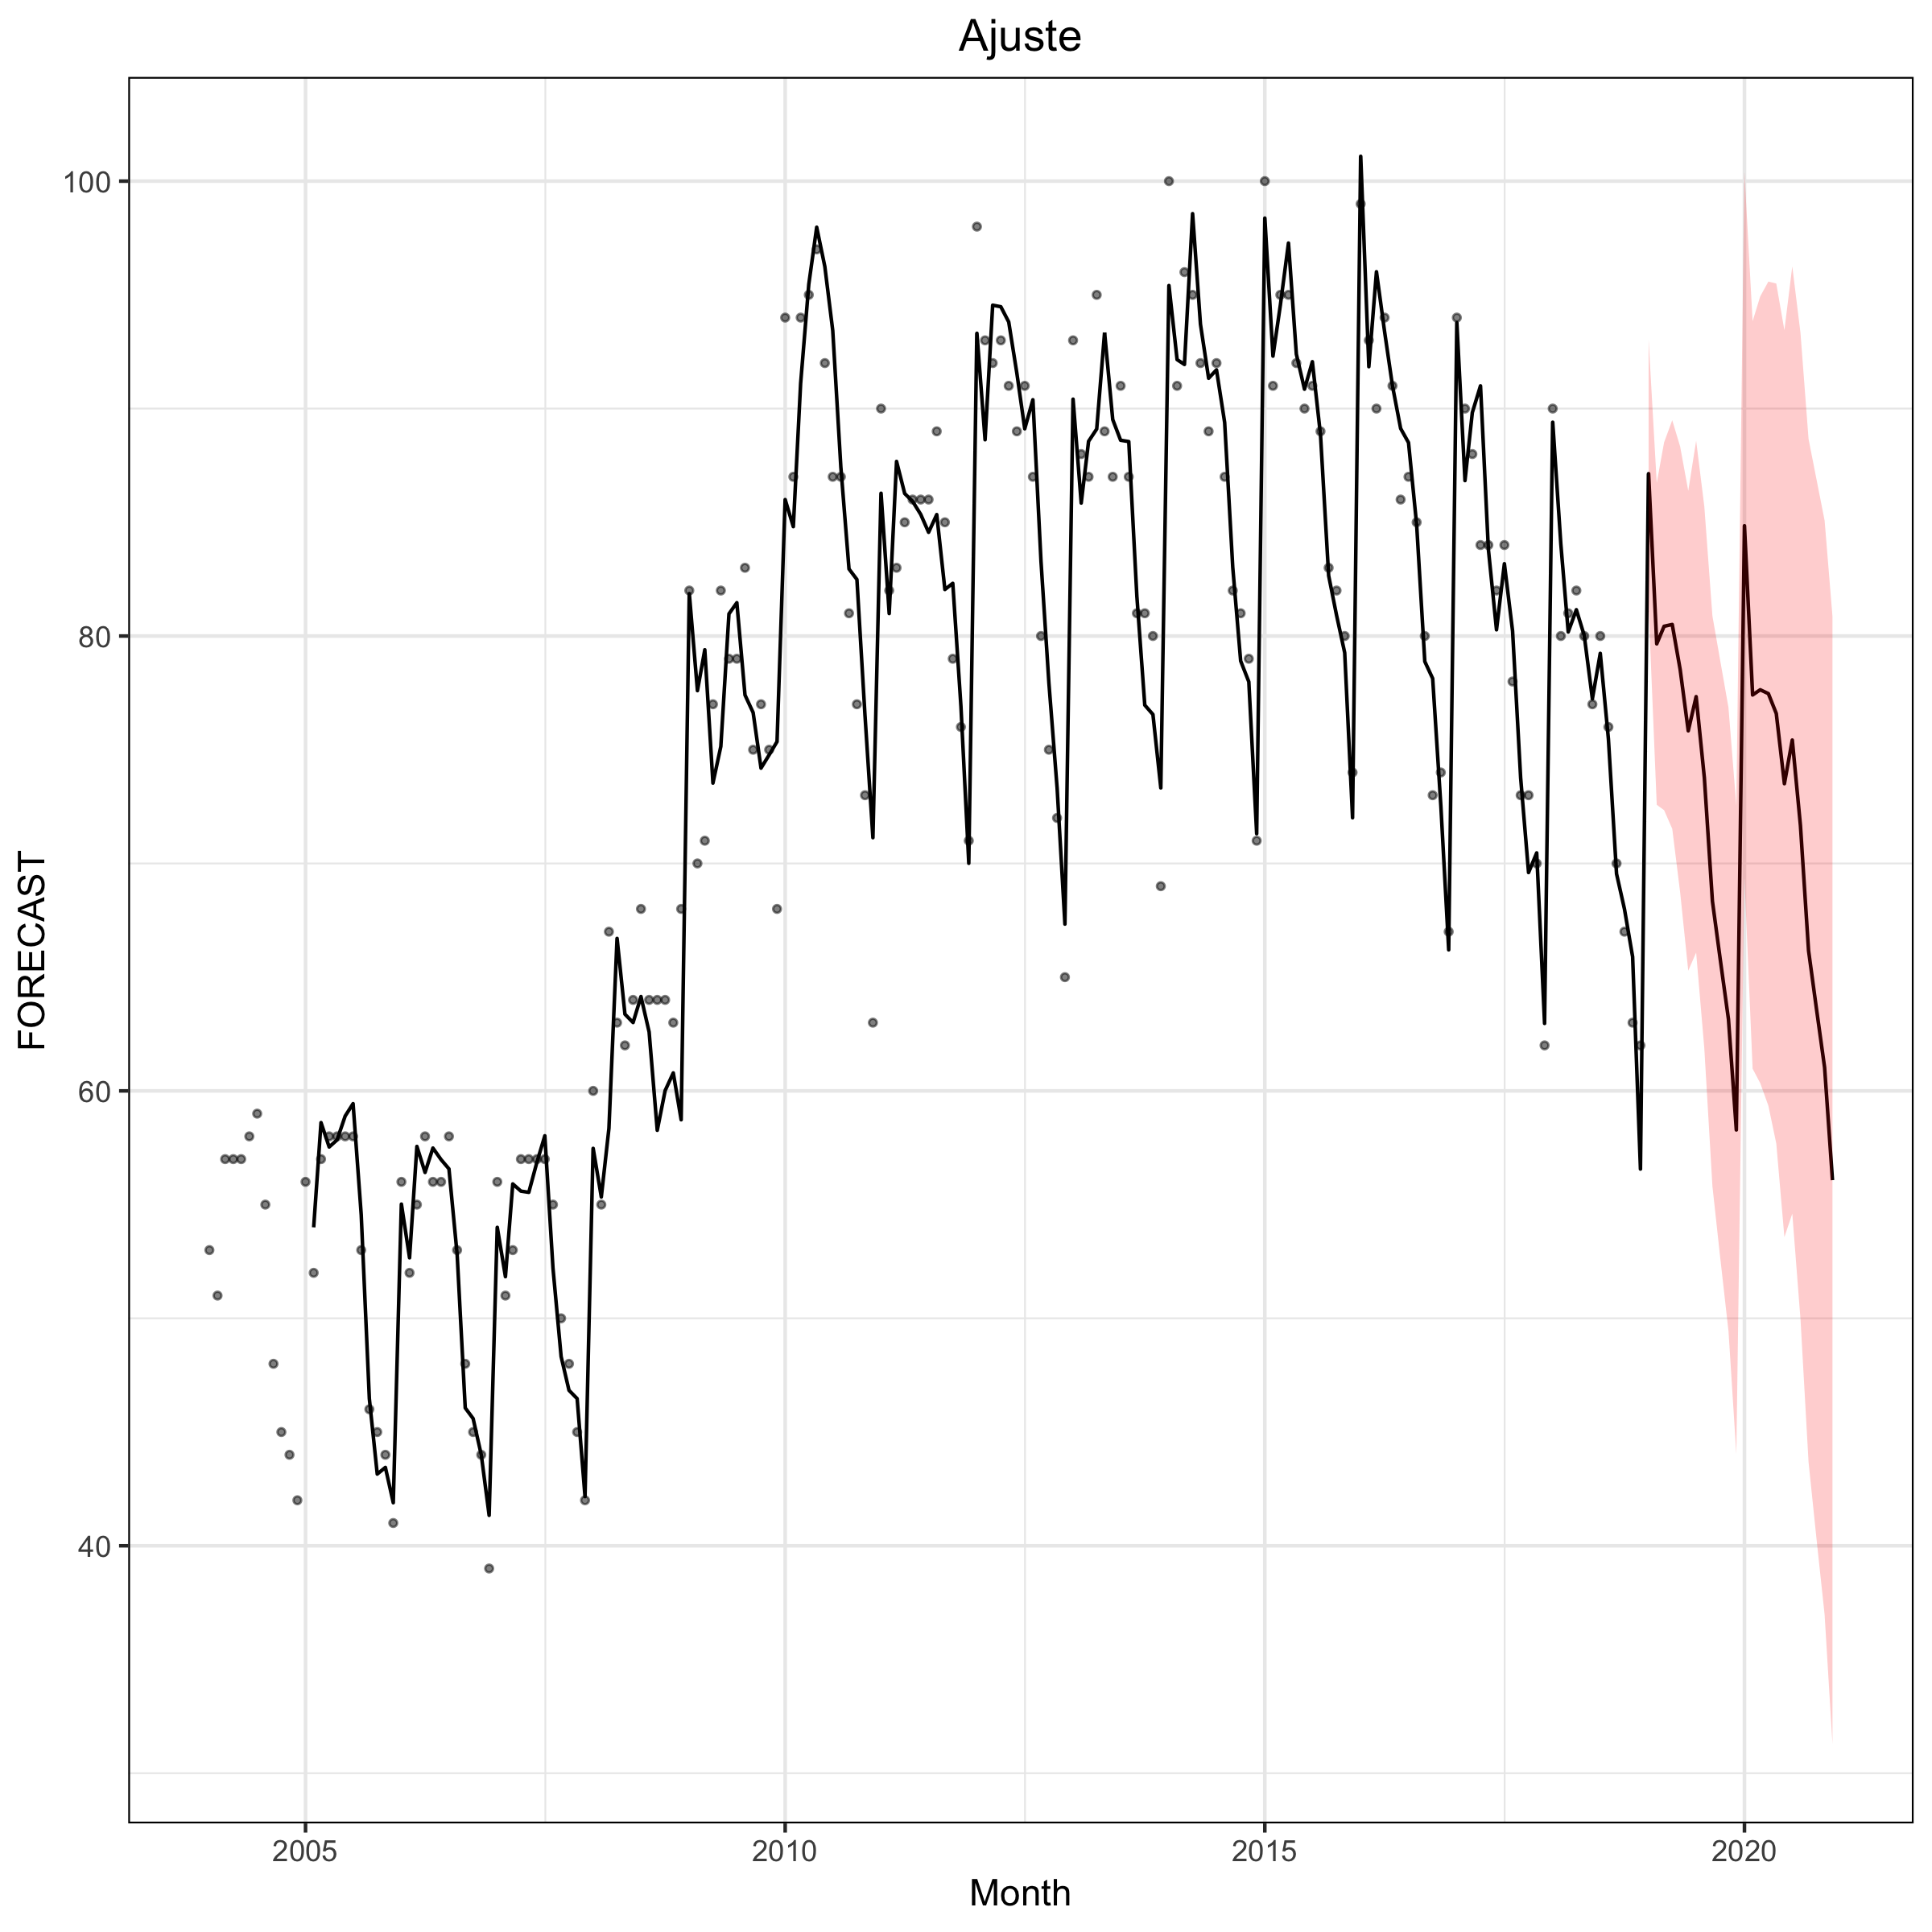
\includegraphics[width=0.7\textwidth]{predict-complete}
      \caption{Predicción $24$ observaciones hacia delante de la serie \texttt{weightloss} utilizando el modelo $\text{SARIMA}(0, 1, 1)(0, 1, 1)_{12}(0, 0, 1)_{17}$. (Serie completa)}
      \label{img:predict_complete}
    \end{figure}

    \paragraph{}
    [TODO]

    \begin{figure}[htb!]
      \centering
      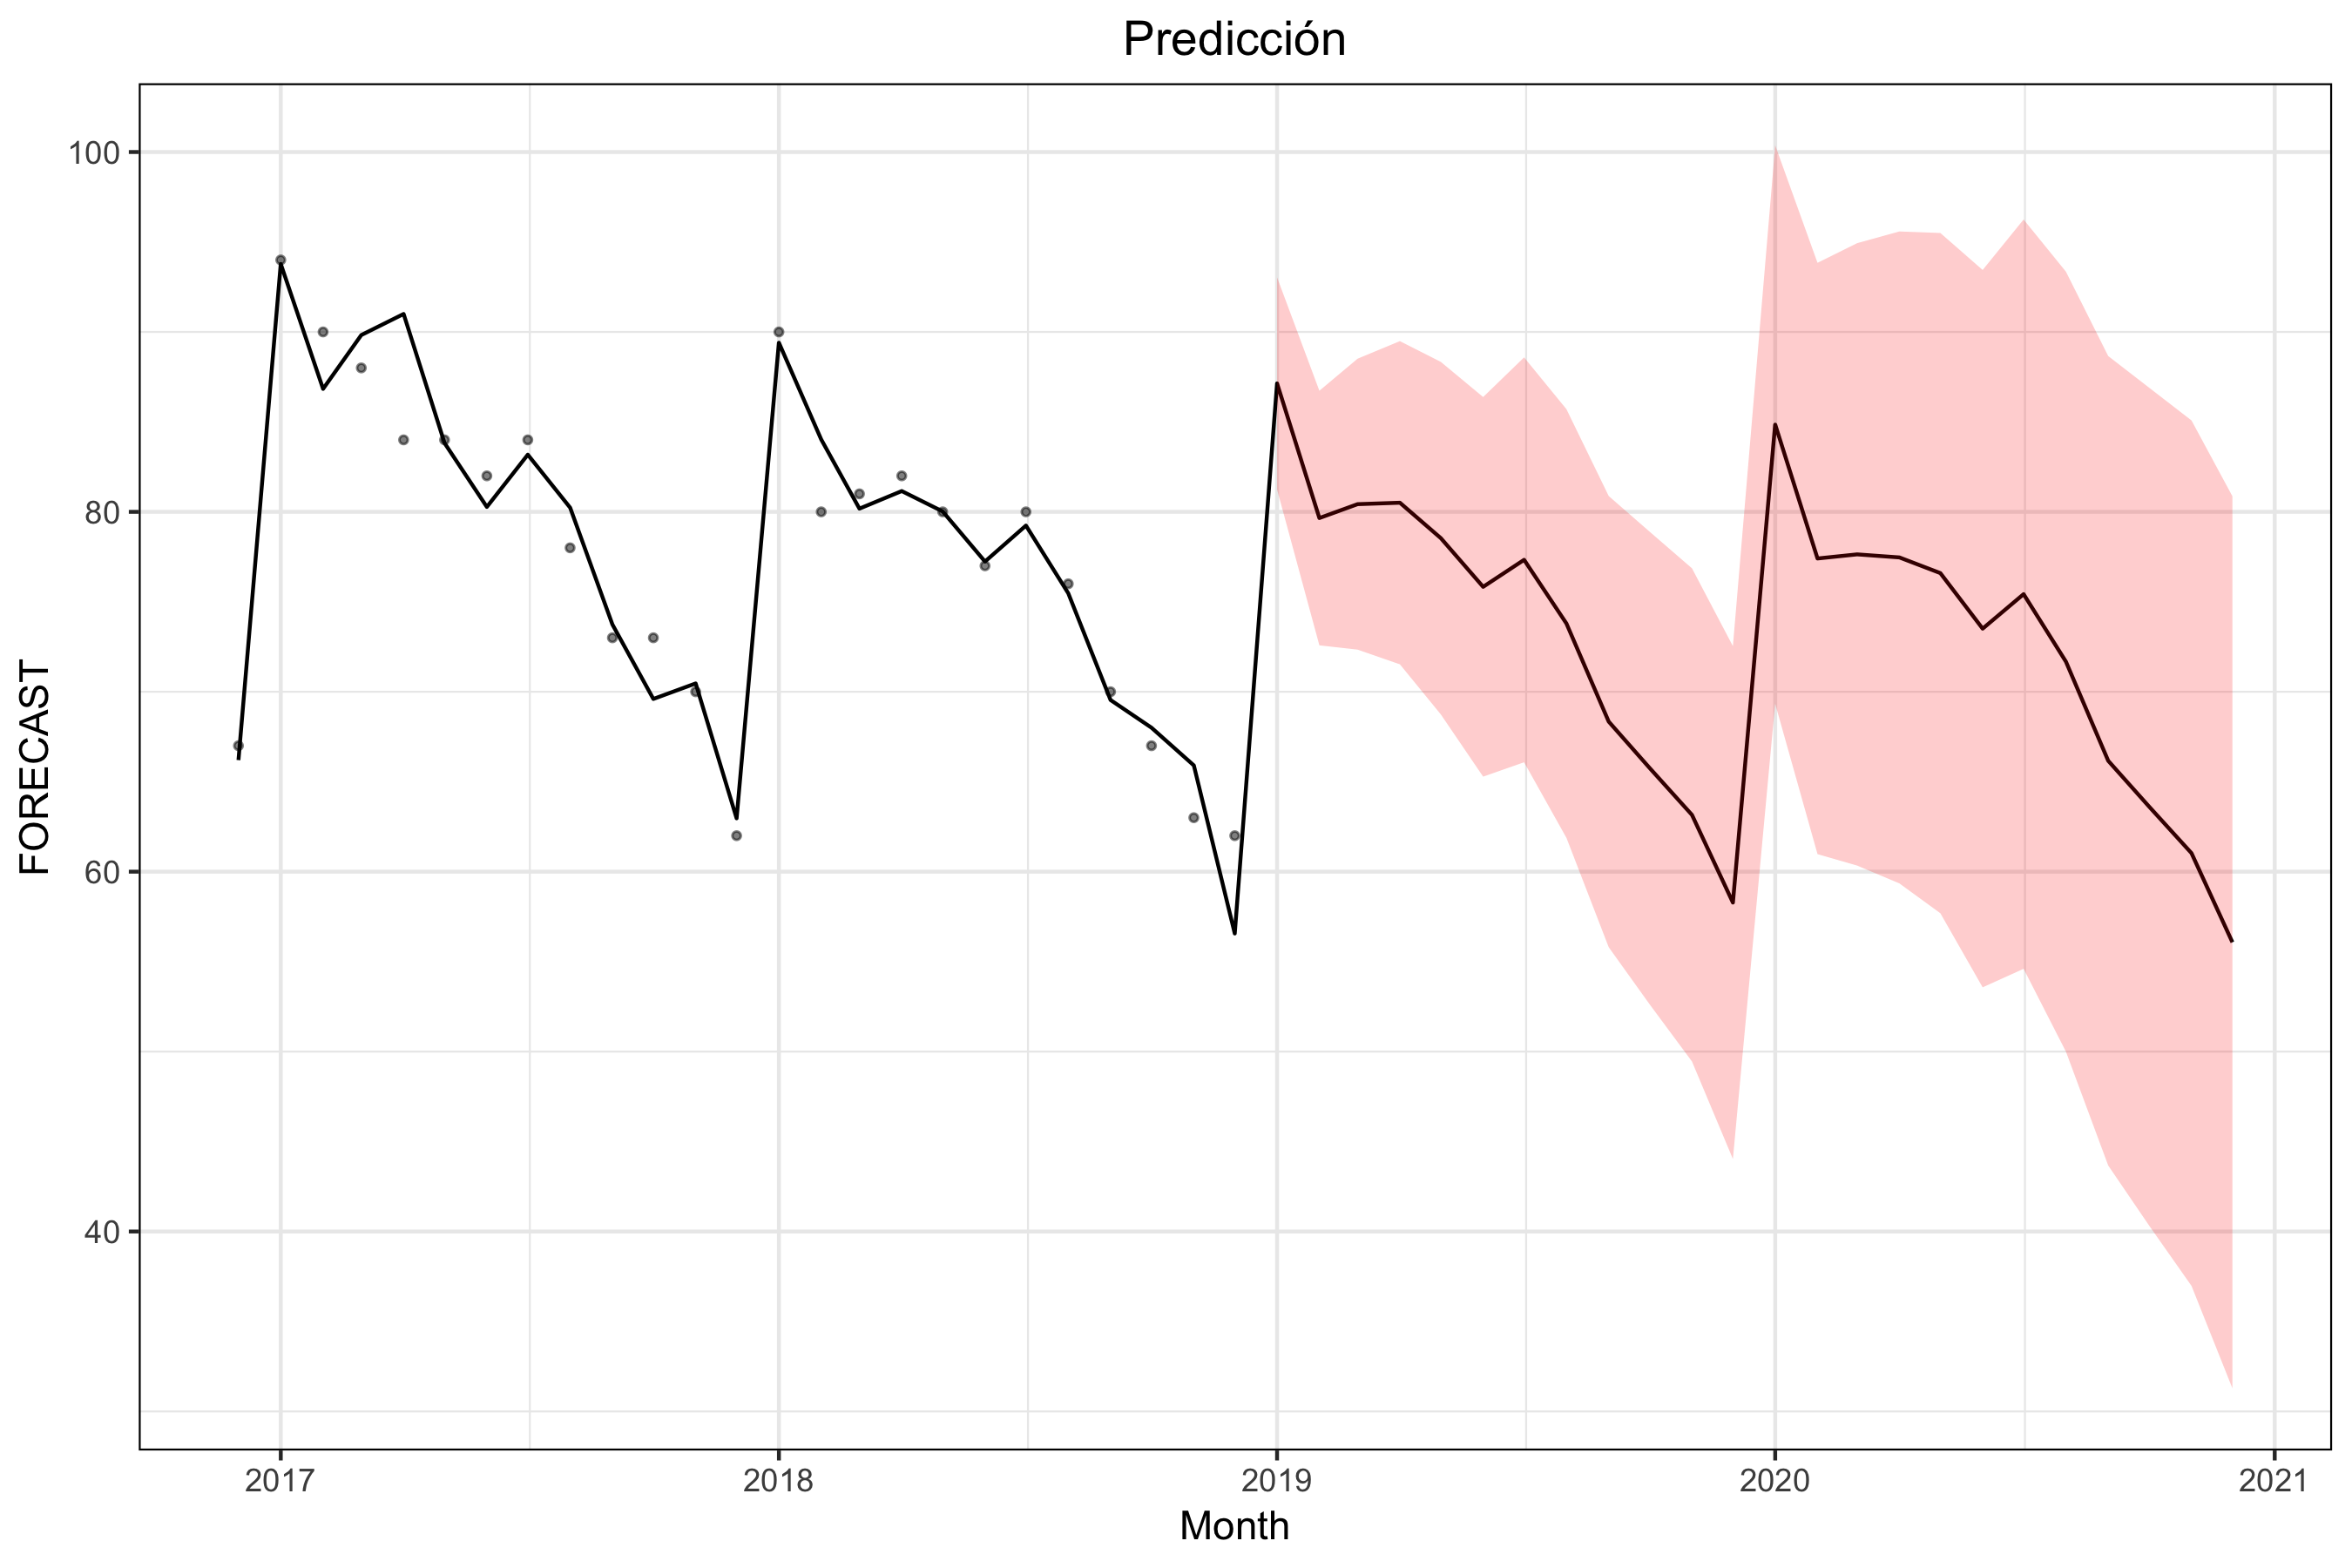
\includegraphics[width=0.7\textwidth]{predict-ending}
      \caption{Predicción $24$ observaciones hacia delante de la serie \texttt{weightloss} utilizando el modelo $\text{SARIMA}(0, 1, 1)(0, 1, 1)_{12}(0, 0, 1)_{17}$. (Últimas observaciones de la serie)}
      \label{img:predict_ending}
    \end{figure}

    \paragraph{}
    [TODO]

  \appendix
  \section{Código Fuente}
  \label{sec:code}

    \begin{listing}[H]
      \centering
      \inputminted{R}{./res/code/functions.r}
      \caption{Conjunto de funciones de apoyo necesarias para el análisis descriptivo de series temporales utilizando el lenguaje \texttt{R}.}
      \label{code:functions_r}
    \end{listing}

    \begin{listing}[H]
      \centering
      \inputminted{R}{./res/code/plotting.r}
      \caption{Función de generación de representación gráfica de una serie utilizando el lenguaje \texttt{R}.}
      \label{code:plotting_r}
    \end{listing}

    \begin{listing}[H]
      \centering
      \inputminted{R}{./res/code/descriptive.r}
      \caption{Análisis descriptivo utilizando el lenguaje \texttt{R} de la serie \texttt{weightloss}.}
      \label{code:descriptive_r}
    \end{listing}

    \begin{listing}[H]
      \centering
      \inputminted{SAS}{./res/code/import.SAS}
      \caption{Importación de datos utilizando el lenguaje \texttt{SAS} del conjunto de datos para la serie \texttt{weightloss}.}
      \label{code:import_sas}
    \end{listing}

    \begin{listing}[H]
      \centering
      \inputminted{SAS}{./res/code/validation_1.sas}
      \caption{Validación utilizando el lenguaje \texttt{SAS} del modelo $\text{SARIMA}(0, 1, 1)(0, 1, 1)_{12}$ sobre la serie \texttt{weightloss}.}
      \label{code:validation_1_sas}
    \end{listing}

    \begin{listing}[H]
      \centering
      \inputminted{R}{./res/code/validation_1.r}
      \caption{Validación utilizando el lenguaje \texttt{R} del modelo $\text{SARIMA}(0, 1, 1)(0, 1, 1)_{12}$ sobre la serie \texttt{weightloss}.}
      \label{code:validation_1_r}
    \end{listing}

    \begin{listing}[H]
      \centering
      \inputminted{SAS}{./res/code/validation_2.sas}
      \caption{Validación utilizando el lenguaje \texttt{SAS} del modelo $\text{SARIMA}(0, 1, 1)(0, 1, 1)_{12}(0, 0, 1)_{17}$ sobre la serie \texttt{weightloss}.}
      \label{code:validation_2_sas}
    \end{listing}

    \begin{listing}[H]
      \centering
      \inputminted{R}{./res/code/validation_2.r}
      \caption{Validación utilizando el lenguaje \texttt{R} del modelo $\text{SARIMA}(0, 1, 1)(0, 1, 1)_{12}(0, 0, 1)_{17}$ sobre la serie \texttt{weightloss}.}
      \label{code:validation_2_r}
    \end{listing}


    \begin{listing}[H]
      \centering
      \inputminted{SAS}{./res/code/validation_3.sas}
      \caption{Validación utilizando el lenguaje \texttt{SAS} del modelo $\text{SARIMA}(1, 1, 1)(0, 1, 1)_{12}$ sobre la serie \texttt{weightloss}.}
      \label{code:validation_3_sas}
    \end{listing}

    \begin{listing}[H]
      \centering
      \inputminted{SAS}{./res/code/validation_4.sas}
      \caption{Validación utilizando el lenguaje \texttt{SAS} del modelo $\text{SARIMA}(1, 1, 1)(0, 1, 1)_{12}(0, 0, 1)_{17}$ sobre la serie \texttt{weightloss}.}
      \label{code:validation_4_sas}
    \end{listing}

    \begin{listing}[H]
      \centering
      \inputminted{SAS}{./res/code/comparison.sas}
      \caption{Comparación utilizando el lenguaje \texttt{SAS} entre los modelos $\text{SARIMA}(0, 1, 1)(0, 1, 1)_{12}$ y $\text{SARIMA}(0, 1, 1)(0, 1, 1)_{12}(0, 0, 1)_{17}$ sobre la serie \texttt{weightloss}.}
      \label{code:comparison_sas}
    \end{listing}

    \begin{listing}[H]
      \centering
      \inputminted{R}{./res/code/comparison.r}
      \caption{Comparación utilizando el lenguaje \texttt{R} entre los modelos $\text{SARIMA}(0, 1, 1)(0, 1, 1)_{12}$ y $\text{SARIMA}(0, 1, 1)(0, 1, 1)_{12}(0, 0, 1)_{17}$ sobre la serie \texttt{weightloss}.}
      \label{code:comparison_r}
    \end{listing}

    \begin{listing}[H]
      \centering
      \inputminted{SAS}{./res/code/predict.sas}
      \caption{Cálculo de la predicción utilizando el lenguaje \texttt{SAS} de las $24$ observaciones siguientes utilizando el modelo $\text{SARIMA}(0, 1, 1)(0, 1, 1)_{12}(0, 0, 1)_{17}$ sobre la serie \texttt{weightloss}.}
      \label{code:predict_sas}
    \end{listing}

\end{document}
